\documentclass[12pt,a4paper]{article}

% Packages
\usepackage[utf8]{inputenc}
\usepackage[T1]{fontenc}
\usepackage{amsmath,amssymb,amsthm}
\usepackage{mathtools}
\usepackage{geometry}
\usepackage{graphicx}
\usepackage{hyperref}
\usepackage{cleveref}
\usepackage{enumitem}
\usepackage{physics}

% Page geometry
\geometry{
    margin=1in,
    headheight=15pt
}

% Theorem environments
\newtheorem{theorem}{Theorem}[section]
\newtheorem{lemma}[theorem]{Lemma}
\newtheorem{proposition}[theorem]{Proposition}
\newtheorem{corollary}[theorem]{Corollary}
\theoremstyle{definition}
\newtheorem{definition}[theorem]{Definition}
\newtheorem{example}[theorem]{Example}
\theoremstyle{remark}
\newtheorem{remark}[theorem]{Remark}

% Custom commands
\newcommand{\Nmax}{N_{\text{max}}}

% Hyperref setup
\hypersetup{
    colorlinks=true,
    linkcolor=blue,
    citecolor=blue,
    urlcolor=blue
}

\title{\textbf{On the Consequences of Observation: Deriving Properties of the  The Observation Boundary Through Categorical Enumeration at Cosmic Heat Death}}

\author{Kundai Farai Sachikonye}

\date{\today}

\begin{document}

\maketitle

\begin{abstract}
We present a rigorous method for counting the maximum number of categorical distinctions that can be made in the observable universe. By analyzing the heat death configuration, where approximately $10^{80}$ particles are maximally separated, we derive a recursive formula $C(t+1) = n^{C(t)}$ that governs the growth of categorical complexity. This recursion produces tetration with base $n \approx 10^{84}$ and depth $t \approx 10^{80}$, yielding $\Nmax \approx (10^{84}) \uparrow\uparrow (10^{80})$.

This number exceeds all previously known large numbers to such an extreme degree that every other number—including Graham's number, TREE(3), and any combination thereof—becomes effectively zero in comparison. Specifically, we prove that even if one uses TREE(3) as the base of a counting system and counts for the maximum computationally allowed operations ($\sim 10^{120}$) over the universe's lifetime, the result is negligible compared to $\Nmax$. This establishes $\Nmax$ as a unique magnitude threshold.

The counting procedure requires accounting for observer networks, since categorical distinctions exist only relative to observers who make them. Crucially, categories arise because observers have preferences (goals, needs) and must organize information to achieve them. The universe itself makes no distinctions; only observers with purposes impose categorical structure onto undifferentiated reality.

Through this analysis, we find that the maximum categorical complexity naturally expresses in the form $\infty - x$ from any observer's perspective, where $x$ represents information inaccessible to that observer. The magnitude of $\Nmax$ makes this structure necessary rather than optional: since all finite reference points become zero relative to $\Nmax$, embedded observers must experience it as effectively infinite. Furthermore, $x$ arises necessarily because different observers with different goals impose incompatible categorical structures, making some information inaccessible.

Notably, the ratio $x/(\infty - x) \approx 5.4$ emerges from the counting procedure and corresponds to the observed ratio of dark matter to ordinary matter. We present this correspondence without claiming causation, noting that our primary contribution is combinatorial: establishing rigorous bounds on categorical enumeration in a finite universe.
\end{abstract}

\tableofcontents
\newpage

% ============================================================================
% SECTION 1: INTRODUCTION
% ============================================================================
\section{Introduction}

The question "What is the largest number?" admits multiple interpretations. One can ask about the largest number expressible in a given notation, the largest number definable in a formal system, or the largest number of distinct states accessible to a physical system. We pursue a different approach: counting the maximum number of categorical distinctions that can be made by observers attempting to enumerate all possible configurations of matter at the heat death of the universe.

This problem is not merely philosophical. At heat death, the universe reaches maximum entropy with particles maximally separated~\cite{PenroseRoadToReality}. Each particle (e.g., an oxygen molecule with $\sim 25{,}000$ vibrational modes) can exist in numerous distinct configurations. The spaces between particles also possess structure describable in terms of field configurations. A rigorous enumeration of all distinguishable configurations at this state yields a well-defined, though incomprehensibly large, finite number.

The counting procedure reveals unexpected mathematical structure. Because observers can only access partial information about the system, with full reconstruction requiring integration of multiple observer perspectives, the enumeration produces a recursion of the form $C(t+1) = n^{C(t)}$, characteristic of tetration. This yields $\Nmax \approx (10^{84}) \uparrow\uparrow (10^{80})$, a number so large that all other known large numbers become effectively zero in comparison—a result we prove rigorously in Section 5.

Furthermore, from any single observer's perspective, the total appears in the form $\infty - x$, where $x$ represents information inaccessible to that observer. The extreme magnitude of $\Nmax$ makes this structure necessary: when every finite number is negligible compared to the total, embedded observers cannot distinguish the total from infinity. The $\infty - x$ structure is thus an arithmetic consequence, not a philosophical choice.

We emphasize at the outset that our approach is combinatorial. We do not propose a physical theory of dark matter, consciousness, or quantum mechanics. Rather, we count carefully and report what emerges from that counting. That the results correspond to observed physical quantities (e.g., dark matter ratio $\sim 5.4$) is noteworthy and merits further investigation by specialists in those domains.

% ============================================================================
% SECTION 2: OBSERVATION REQUIREMENTS
% ============================================================================
\section{Observation and Categorical Distinction}
To count categorical distinctions, we must first establish what constitutes a "distinction." In this work, we adopt an operational definition: a categorical distinction exists if and only if an observer can differentiate between two configurations through measurement or observation.

\subsection{The Role of Observers}

\begin{definition}[Observer]
An \emph{observer} is a physical system capable of making measurements that distinguish between different configurations of other systems. Formally, an observer $O$ possesses:
\begin{enumerate}[label=(\roman*)]
    \item A measurement apparatus with finite resolution
    \item A memory system to record measurement outcomes
    \item An internal state that changes in response to observations
\end{enumerate}
\end{definition}

Observers are necessary for categorical distinction because physical configurations do not inherently partition themselves. A molecule in one vibrational state versus another represents two "different" configurations only if some system can distinguish between them. Without observers, there are no categories—only undifferentiated physical reality.

\subsection{Observation Requires Termination}

A crucial constraint governs observation: to observe a system's state, the observation process must complete (terminate). This is not merely a practical limitation but follows from information theory.

\begin{proposition}[Observation Termination]
Let $O$ be an observer attempting to measure system $S$. The measurement produces a definite outcome only when the interaction between $O$ and $S$ is complete, establishing a correlated state $O \otimes S$ in which $O$'s memory encodes information about $S$.
\end{proposition}

Incomplete or ongoing processes cannot be observed because they do not yet have definite outcomes. This has important consequences: if a process never terminates, it remains unobservable, contributing no categorical distinctions to our count.

\begin{figure*}[htbp]
    \centering
    \includegraphics[width=0.95\textwidth]{figures/observer_dependent_structure.png}
    \caption{\textbf{Observer-dependent categorical structure and $\infty - x$ framework.}
    \textbf{Top:} Observable $\infty - x$ (blue curve with circles) increases from $\approx 0$ to $\approx 1.2$ while inaccessible $x$ (red curve with squares) decreases from $\approx 1.0$ to $\approx 0$ as observer count grows from 0 to 50. Curves cross at $\approx 20$ observers where observable and inaccessible fractions are equal.
    \textbf{Middle-left:} Ratio $x/(\infty - x)$ (purple curve with triangles) versus number of observers shows rapid decay from $\approx 10$ at 5 observers to $\approx 0.5$ at 30 observers. Green dashed line marks observed dark matter ratio $\approx 5.4$; intersection occurs at $\approx 10$ observers.
    \textbf{Middle-right:} Convergence analysis shows $|\text{Ratio} - 5.4|$ on log scale versus number of observers. Error drops from $\approx 10^3$ at 5 observers to minimum $\approx 10^{-1}$ at $\approx 10$ observers (red circles), then stabilizes.
    \textbf{Bottom-left:} Observer network diagram shows 5 observers O1-O5 (blue circles) connected by dashed lines representing mutual observation. Recursive constraint: observers must observe observers; no single observer accesses complete information.
    \textbf{Bottom-right:} Key insights box (cyan) summarizes $\infty - x$ structure: Observable $= \infty - x$, Inaccessible $= x$, Ratio $x/(\infty - x) = 5.4$. Physical correspondence to dark matter:ordinary matter ratio $= 5.4:1$ emerges from counting; correspondence presented without claiming causation.
    \textbf{Bottom banner:} Orange disclaimer states analysis is purely combinatorial. Categorical distinctions counted and emergent ratios reported; physical interpretation left to domain specialists.}
    \label{fig:observer_dependent}
\end{figure*}

\subsection{Partial Information and Observer Networks}

No single observer can access complete information about a macroscopic system. Each observer has:
\begin{itemize}
    \item \textbf{Finite spatial range:} Cannot observe arbitrarily distant regions
    \item \textbf{Finite temporal range:} Finite lifetime bounds observation duration
    \item \textbf{Finite resolution:} Cannot distinguish arbitrarily fine differences
\end{itemize}

To reconstruct complete system information, it is necessary to integrate observations from multiple observers. However, other observers are themselves physical systems that must be observed. This creates recursive structure: to know the complete state requires observing all observers, including the observer doing the observing.

\begin{definition}[Observer Network]
An \emph{observer network} $\mathcal{N} = \{O_1, O_2, \ldots, O_N\}$ is a collection of $N$ observers, each of which observes:
\begin{enumerate}[label=(\roman*)]
    \item Some portion of the physical system
    \item Some subset of other observers in $\mathcal{N}$
\end{enumerate}
\end{definition}

Complete information reconstruction requires accounting for all information distributed across the observer network, including information about which observers observed which parts of the system.

\subsection{Categories as Observer-Dependent Distinctions}

We formalize categorical distinctions as follows:

\begin{definition}[Category]
Given an observer network $\mathcal{N}$ at time $t$, a \emph{category} $C$ is an equivalence class of physical configurations that cannot be distinguished by any observer in $\mathcal{N}$ given their collective observations up to time $t$.
\end{definition}

Two configurations belong to the same category if no observer in the network can tell them apart. They belong to different categories if at least one observer can distinguish them.

The number of categories $C(t)$ at time $t$ equals the number of distinguishable equivalence classes. This number depends on:
\begin{itemize}
    \item The physical configuration of the system
    \item The number and capabilities of observers
    \item The history of observations made
\end{itemize}

Crucially, categories proliferate as observers proliferate and as the history of observation lengthens, because new distinctions become possible. This proliferation follows mathematical rules we derive in subsequent sections.


% ============================================================================
% SECTION 3: COSMOLOGICAL FRAMEWORK
% ============================================================================
\section{The Heat Death Configuration}
We apply the counting framework to a specific physical configuration: the heat death state of the universe. This provides well-defined boundary conditions and allows concrete estimation of categorical complexity.

\subsection{Heat Death as Maximum Entropy State}

At heat death, the universe reaches maximum entropy~\cite{PenroseRoadToReality}. All thermodynamic gradients have dissipated, and matter exists in a state of maximum

 spatial dispersion. Current cosmological estimates suggest:

\begin{itemize}
    \item \textbf{Particle number:} $N_{\text{particles}} \approx 10^{80}$ (primarily photons, neutrinos, and remnant baryonic matter)
    \item \textbf{Average separation:} $\langle r \rangle \sim 10^{26}$ m (horizon-scale distances)
    \item \textbf{Temperature:} $T \to 0$ K (asymptotically)
    \item \textbf{Expansion:} Continues indefinitely under dark energy domination
\end{itemize}

This configuration is optimal for categorical counting because maximum separation implies maximum potential for independent observations: each particle can, in principle, be observed independently by a separate observer.

\begin{figure*}[htbp]
    \centering
    \includegraphics[width=0.95\textwidth]{figures/heat_death_enumeration.png}
    \caption{\textbf{Heat death categorical enumeration.}
    \textbf{Top:} Recursive categorical enumeration shows $\log_{10}(\text{Categorical Count})$ versus depth $t$ following tetration growth $C(t+1) = n^{C(t)}$ (purple curve). Growth accelerates dramatically from $\log_{10}(C(t)) \approx 1$ at $t=0$ to $\approx 10$ at $t=1$, exceeding Graham's number.
    \textbf{Bottom-left:} Comparison bar chart shows $\log_{10}(\text{Number})$ for Googol ($10^{100}$), Googolplex ($10^{\text{googol}}$), Graham's Number, TREE(3), and this work. $N_{\max}$ (green bar, $\approx 100$) exceeds all previous large numbers by orders of magnitude.
    \textbf{Center:} Heat death configuration shows 8 maximally separated particles (P1-P8, red circles) around observer (blue star). Configuration represents $\sim 10^{80}$ particles each with $\sim 25{,}000$ distinguishable modes, yielding base $n \approx 10^{80} \times 25{,}000$ for tetration.
    \textbf{Bottom-right:} Observer network complexity (blue curve) versus number of observers shows super-linear growth from $\approx 0$ at 2 observers to $\approx 220$ at 20 observers. Table lists parameters: particles $\sim 10^{80}$, modes per particle $\sim 25{,}000$, recursion $C(t+1) = n^{C(t)}$, growth type tetration, exceeds Graham's number, form $\infty - x$.
    \textbf{Methodology:} Five-step procedure: (1) start with heat death configuration, (2) count distinguishable modes per particle, (3) apply recursive enumeration, (4) account for observer networks, (5) result yields tetration growth. Rigorous counting produces number so large it motivates $\infty - x$ structure where $N_{\max}$ appears as infinity minus inaccessible information.}
    \label{fig:heat_death_enumeration}
\end{figure*}

\subsection{Particle Configurational States}

Each particle possesses internal degrees of freedom that constitute distinguishable configurations. Consider a molecular example:

\begin{example}[Oxygen Molecule]
\label{ex:oxygen_molecule}
An O$_2$ molecule has approximately $25{,}000$ distinct vibrational modes arising from:
\begin{itemize}
    \item Symmetric and antisymmetric stretching modes
    \item Rotational states (quantized angular momentum)
    \item Electronic state configurations
\end{itemize}
At any given moment, the molecule occupies one specific configuration. Changing to a different configuration represents a distinguishable categorical state.
\end{example}

For our counting, we estimate:
\begin{equation}
n_{\text{particle}} \approx 10^4 \text{ distinguishable configurations per particle}
\end{equation}

This is a conservative lower bound. More complex molecules or systems would have larger configuration spaces.

\subsection{Field Configurations in Empty Space}

The space between particles is not empty but filled with quantum fields (electromagnetic, gravitational, etc.). These fields possess their own configurational states.

From an observer stationed "inside" a region of space looking outward, the field configuration at the boundary resembles the electron cloud of an atom: there is surface structure without a central nucleus (particles being distant). This field structure is distinguishable and must be counted.

The number of distinguishable field configurations in each inter-particle region is comparable to particle configurations:
\begin{equation}
n_{\text{space}} \approx 10^4 \text{ distinguishable field configurations}
\end{equation}

Since there are approximately as many inter-particle regions as particles (in a maximally dispersed configuration), the total number of distinguishable entities is:
\begin{equation}
N_{\text{total}} = N_{\text{particles}} + N_{\text{spaces}} \approx 2 \times 10^{80}
\end{equation}

\subsection{Observer Distribution at Heat Death}

To observe all particles independently requires observers distributed throughout the volume. Given horizon constraints (observers cannot see beyond their cosmological horizon), we require:
\begin{equation}
N_{\text{observers}} \sim N_{\text{particles}} \sim 10^{80}
\end{equation}

Each observer can observe their local neighborhood but requires information from other observers to reconstruct the global state. This observer network structure is crucial for the recursive counting that follows.

\subsection{Total Configuration Parameter}

For the recursive enumeration in Section~\ref{sec:recursion}, we require a base parameter $n$ representing the number of distinguishable alternatives at each categorical level:
\begin{equation}
n = N_{\text{total}} \times n_{\text{configs}} \approx (2 \times 10^{80}) \times (10^4) \approx 10^{84}
\end{equation}

This represents the total number of entity-configuration pairs: each of $2 \times 10^{80}$ entities (particles and spaces) can be in one of $10^4$ configurations.

\subsection{Physical Bounds}

Several physical principles constrain the maximum categorical complexity:

\begin{enumerate}[label=(\alph*)]
    \item \textbf{Holographic bound~\cite{tHooft1993,Susskind1995}:} Maximum information content scales with surface area, not volume:
    \begin{equation}
    I_{\max} = \frac{A}{4\ell_P^2} \approx 10^{122} \text{ bits}
    \end{equation}
    where $\ell_P \approx 1.6 \times 10^{-35}$ m is the Planck length.

    \item \textbf{Margolus-Levitin bound~\cite{Margolus1998}:} Maximum computational operations over cosmic timescales:
    \begin{equation}
    N_{\text{ops}} \leq \frac{E t_{\text{universe}}}{\hbar} \approx 10^{120}
    \end{equation}

    \item \textbf{Bekenstein bound~\cite{Bekenstein1981}:} Maximum entropy for finite energy and radius:
    \begin{equation}
    S_{\max} \leq \frac{2\pi k_B R E}{\hbar c} \approx 10^{104} k_B
    \end{equation}
\end{enumerate}

These bounds will constrain the maximum value of $C(t)$ we can physically realize, though our counting procedure can formally continue beyond them.


% ============================================================================
% SECTION 4: CATEGORICAL COMPLETION
% ============================================================================
\section{Categorical Accumulation}
%==============================================================================
\section{Categorical Completion in Gas Dynamics}
\label{sec:categorical}
%==============================================================================

\subsection{Categorical State Space}

We now develop the categorical framework for describing gas configurations. This framework extends beyond classical phase space by incorporating phase-lock network topology and oscillatory relationships that are invisible to spatial measurements but fundamental to thermodynamic evolution.

\begin{definition}[Categorical State]
\label{def:categorical_state}
A categorical state $C \in \catspace$ specifies the complete oscillatory and topological structure of a molecular configuration, comprising the phase-lock network topology $\phaselockgraph$, the phase relationships $\{\Delta\phi_{ij}\}$ for all locked pairs, the vibrational mode occupations $\{n_{\text{vib},i}\}$, the rotational state quantum numbers $\{J_i, M_i\}$, and the electronic configuration descriptors.
\end{definition}

\begin{remark}
A categorical state contains strictly more information than a classical phase space point $(\mathbf{q}, \mathbf{p})$. Two configurations with identical positions and momenta can occupy different categorical states if their phase relationships or network topologies differ. This additional structure is not merely mathematical bookkeeping but reflects physical reality: molecules with identical spatial configurations but different phase relationships have different interaction energies, different spectroscopic signatures, and different dynamical evolution. The categorical state captures the full oscillatory context that determines thermodynamic behavior.
\end{remark}

\begin{definition}[Categorical State Space]
\label{def:categorical_state_space}
The categorical state space $\catspace$ is the set of all categorical states equipped with a partial order $\prec$ called the completion order, a completion operator $\mu: \catspace \times \mathbb{R}_{\geq 0} \to \{0, 1\}$ indicating whether state $C$ has been occupied by time $t$, and a topology $\tau$ induced by $\prec$ that makes categorical adjacency continuous.
\end{definition}

The completion operator $\mu(C, t) = 1$ indicates that categorical state $C$ has been occupied (completed) by time $t$, while $\mu(C, t) = 0$ indicates it remains unoccupied. This binary distinction captures the fundamental irreversibility of categorical completion: once a state is occupied, it remains in the system's history.

\begin{axiom}[Categorical Irreversibility]
\label{axiom:categorical_irreversibility}
Once a categorical state $C_i$ is occupied, it cannot be re-occupied. For all $C_i \in \catspace$ and times $t_1 \leq t_2$:
\begin{equation}
\mu(C_i, t_1) = 1 \implies \mu(C_i, t_2) = 1
\label{eq:irreversibility}
\end{equation}
Any process returning to a spatially identical configuration must occupy a new categorical state $C_j$ with $C_i \prec C_j$.
\end{axiom}

This axiom formalises the intuition that time's arrow is encoded in categorical structure. Even when spatial configurations repeat, the phase relationships and network topology have evolved, placing the system in a new categorical state. This is the microscopic origin of thermodynamic irreversibility: not spatial evolution, but categorical completion.

\begin{proposition}[Monotonic Completion]
\label{prop:monotonic_completion}
Let $\gamma(t) = \{C \in \catspace : \mu(C, t) = 1\}$ be the set of completed states at time $t$. Then:
\begin{equation}
t_1 \leq t_2 \implies \gamma(t_1) \subseteq \gamma(t_2)
\end{equation}
The completed set grows monotonically, never contracting.
\end{proposition}

\begin{proof}
Immediate from Axiom~\ref{axiom:categorical_irreversibility}. If $C \in \gamma(t_1)$, then $\mu(C, t_1) = 1$, which implies $\mu(C, t_2) = 1$ for all $t_2 \geq t_1$, hence $C \in \gamma(t_2)$. Therefore $\gamma(t_1) \subseteq \gamma(t_2)$. \qed
\end{proof}

\subsection{Phase-Lock Degeneracy and Categorical Richness}

A crucial insight emerges from the relationship between spatial and categorical descriptions: a single spatial configuration corresponds to many categorical states. This degeneracy is not a deficiency of the categorical framework but rather reveals hidden structure invisible to spatial measurements.

\begin{theorem}[Phase-Lock Degeneracy]
\label{thm:phase_lock_degeneracy}
For a spatial configuration $\mathbf{q} = \{\mathbf{r}_1, \ldots, \mathbf{r}_N\}$, there exist multiple categorical states producing identical spatial observables. The phase-lock degeneracy is:
\begin{equation}
\Omega_{\text{PL}}(\mathbf{q}) = |\{C \in \catspace : \pi_{\text{spatial}}(C) = \mathbf{q}\}|
\label{eq:phase_lock_degeneracy}
\end{equation}
where $\pi_{\text{spatial}}: \catspace \to \mathbb{R}^{3N}$ is the spatial projection.
\end{theorem}

\begin{proof}
Consider two molecules at fixed positions $\mathbf{r}_1$ and $\mathbf{r}_2$ separated by distance $r_{12}$. The same spatial configuration can be achieved through different combinations of oscillatory phases. Van der Waals interactions have no preferred angular orientation, contributing a continuous degeneracy. For molecules with permanent dipoles, the orientations $(\theta_1, \phi_1)$ and $(\theta_2, \phi_2)$ can vary while maintaining the same spatial positions, provided the molecular centers remain fixed. Vibrational phases $\phi_{\text{vib},i}$ are independent degrees of freedom not specified by spatial position. Rotational phases $\phi_{\text{rot},i}$ similarly vary independently of molecular center-of-mass location.

These constitute distinct categorical states with different phase relationships $\{\Delta\phi_{ij}\}$ but identical spatial projection $\pi_{\text{spatial}}(C) = \mathbf{q}$.

For $N$ molecules with $\binom{N}{2}$ pairwise interactions, each having $k$ independent phase degrees of freedom per pair, the degeneracy scales as:
\begin{equation}
\Omega_{\text{PL}}(\mathbf{q}) \sim (2\pi)^{k \cdot \binom{N}{2}}
\end{equation}

For typical molecular gases where $k \approx 3$ to $5$ (vibrational, rotational, and orientational phases), and $N \sim 10^{23}$ molecules in a macroscopic sample, the degeneracy is astronomical. Even for small systems with $N = 100$ molecules, $\Omega_{\text{PL}} \sim 10^6$ to $10^{12}$ per spatial configuration. \qed
\end{proof}

\begin{figure*}[htbp]
\centering
\includegraphics[width=0.95\textwidth]{figures/panel_s_space.png}
\caption{\textbf{S-Entropy Space Visualization: Molecular Distribution in Configurational Entropy Coordinates.}
\textbf{(A)} Molecular distribution in S-space. Three-dimensional visualization of molecular states projected onto entropy coordinates $(S_{\kappa}, S_{\epsilon}, S_t)$, where $S_{\kappa}$ represents kinetic entropy, $S_{\epsilon}$ represents categorical/configurational entropy, and $S_t$ represents topological entropy. Color gradient (purple to yellow) indicates progression through state space. The distribution shows clear clustering structure, with molecules occupying a bounded region of entropy space. The axes span $S_{\kappa} \in [0.96, 1.04]$, $S_{\epsilon} \in [7.5, 10.0]$, and $S_t \in [0.0, 1.0]$, revealing the natural scale separation between different entropy components.
\textbf{(B)} Polar phase diagram: $S_t \to 0$, $S_{\epsilon} \to r$. Radial coordinate represents configurational entropy $S_{\epsilon}$ (ranging from 0 at center to 1.00 at outer edge), while angular coordinate represents phase angle. The distribution (blue line at 0°) shows strong directional preference, indicating phase-locked structure. Concentric circles mark entropy magnitude levels (0.25, 0.50, 0.75, 1.00). The highly anisotropic distribution demonstrates that molecules occupy specific phase relationships, not random orientations, confirming the phase-lock network structure.
\textbf{(C)} Ternary composition diagram. Triangle vertices represent pure states: $S_{\kappa}$ (kinetic, top), $S_{\epsilon}$ (configurational, bottom-left), and $S_t$ (topological, bottom-right). The color bar (blue to red gradient) shows the distribution of molecular states across the three entropy components. Most molecules cluster near the $S_{\epsilon}$ vertex, indicating dominance of configurational entropy. The narrow distribution shows that entropy composition is tightly constrained, not uniformly distributed across the ternary space.
\textbf{(D)} Density contour in $(S_{\kappa}, S_{\epsilon})$ plane. Heat map shows probability density with color scale from 0 (pale yellow) to 35 (dark red). Sharp vertical band at $S_{\kappa} \approx 1.0$ indicates that kinetic entropy is nearly constant across the distribution, while $S_{\epsilon}$ varies from 0.2 to 1.0. The intense red stripe demonstrates that molecules occupy a one-dimensional manifold in the two-dimensional entropy space, revealing strong constraint on accessible states.
\textbf{(E)} Radial distribution function $g(r)$ versus distance from center in entropy space. Peak at $r \approx 0.72$ (height $\approx 35$) indicates strong clustering at specific entropy magnitude. Secondary peaks at $r \approx 0.76$ and $r \approx 0.84$ suggest shell structure in entropy space. The oscillatory pattern demonstrates that molecules do not uniformly fill entropy space but organize into discrete shells, analogous to electron shells in atoms.
\textbf{(F)} Phase trajectories in $(S_{\kappa}, S_t)$ plane. Colored points (ranging from red/orange at bottom to purple at top) trace molecular evolution through entropy space. Trajectories cluster into discrete bands at $S_t \approx 0.0$, $0.2$, $0.4$, $0.6$, $0.8$, and $1.0$, showing quantized topological entropy levels. The vertical alignment indicates that $S_{\kappa}$ remains nearly constant during evolution, while $S_t$ transitions between discrete levels. This reveals that entropy dynamics are dominated by topological transitions, not kinetic changes, supporting the categorical face dominance in Maxwell's demon resolution.}
\label{fig:s_space}
\end{figure*}


\begin{definition}[Categorical Equivalence Class]
\label{def:categorical_equivalence_class}
The categorical equivalence class of state $C$ under spatial observation is:
\begin{equation}
[C]_{\text{spatial}} = \{C' \in \catspace : \pi_{\text{spatial}}(C') = \pi_{\text{spatial}}(C)\}
\end{equation}
States in the same equivalence class are spatially indistinguishable but categorically distinct.
\end{definition}

\begin{corollary}[Categorical Richness]
\label{cor:categorical_richness}
The categorical richness of a spatial configuration is:
\begin{equation}
R(\mathbf{q}) = \log \Omega_{\text{PL}}(\mathbf{q}) = \log |[C]_{\text{spatial}}|
\end{equation}
This quantifies the information content of categorical specification beyond spatial description.
\end{corollary}

The categorical richness $R(\mathbf{q})$ has profound implications for entropy. Traditional statistical mechanics computes entropy by counting spatial configurations accessible at given energy. The categorical framework reveals that each spatial configuration harbors vast additional structure through phase-lock degeneracy. This hidden structure is precisely what categorical completion navigates, and what the Second Law constrains.

\subsection{Categorical Completion Dynamics}

\begin{definition}[Completion Rate]
\label{def:completion_rate}
The categorical completion rate is:
\begin{equation}
\dot{C}(t) = \frac{d|\gamma(t)|}{dt}
\label{eq:completion_rate}
\end{equation}
measuring the rate at which new categorical states are completed.
\end{definition}

\begin{proposition}[Non-Negative Completion Rate]
\label{prop:nonnegative_completion}
For all times $t$:
\begin{equation}
\dot{C}(t) \geq 0
\end{equation}
with equality only when no physical processes occur.
\end{proposition}

\begin{proof}
From Proposition~\ref{prop:monotonic_completion}, $|\gamma(t)|$ is monotonically non-decreasing, hence $\dot{C}(t) = d|\gamma(t)|/dt \geq 0$. Equality $\dot{C}(t) = 0$ requires $|\gamma(t)|$ constant, meaning no new categorical states are completed. This occurs only when the system is frozen in a single categorical state with no dynamical evolution. \qed
\end{proof}

\begin{theorem}[Categorical Completion as Physical Process]
\label{thm:completion_physical}
Every physical process in a gas system corresponds to categorical completion:
\begin{equation}
\text{Process: } \mathbf{q}(t_1) \to \mathbf{q}(t_2) \quad \Longleftrightarrow \quad \text{Completion: } C(t_1) \prec C(t_2)
\end{equation}
The categorical state advances along the completion order, never retreating.
\end{theorem}

\begin{proof}
Consider a gas evolving from configuration $\mathbf{q}(t_1)$ to $\mathbf{q}(t_2)$ over time interval $\Delta t = t_2 - t_1$.

\textbf{Case 1: Distinct spatial configurations where $\mathbf{q}(t_2) \neq \mathbf{q}(t_1)$.}
The new configuration occupies categorical states not accessible from $\mathbf{q}(t_1)$ because the spatial projection differs. By Axiom~\ref{axiom:categorical_irreversibility}, these must be new completions: $C(t_2) \in \gamma(t_2) \setminus \gamma(t_1)$. The categorical state has advanced.

\textbf{Case 2: Identical spatial configurations where $\mathbf{q}(t_2) = \mathbf{q}(t_1)$.}
Even with identical spatial positions, the phase relationships have evolved. During time interval $\Delta t$, molecules undergo vibrational oscillations at frequencies $\omega_{\text{vib}} \sim 10^{13}$ to $10^{14}$ rad/s and rotational motion at frequencies $\omega_{\text{rot}} \sim 10^{11}$ to $10^{12}$ rad/s. The phase differences evolve as:
\begin{equation}
\Delta\phi_{ij}(t_2) = \Delta\phi_{ij}(t_1) + (\omega_i - \omega_j) \Delta t + \text{collision terms}
\end{equation}

For typical $\Delta t \sim 10^{-12}$ s (picosecond timescale), the phase evolution is:
\begin{equation}
|\Delta\phi_{ij}(t_2) - \Delta\phi_{ij}(t_1)| \sim \omega_{\text{vib}} \Delta t \sim 10 \text{ to } 100 \text{ radians}
\end{equation}

The phase relationships have changed substantially despite spatial identity. By Axiom~\ref{axiom:categorical_irreversibility}, return to the original categorical state $C(t_1)$ is impossible. The system occupies a new state $C(t_2)$ with $C(t_1) \prec C(t_2)$.

\textbf{Case 3: Thermal fluctuations returning to previous spatial configuration.}
Consider a molecule that moves from position $\mathbf{r}_i(t_1)$ to $\mathbf{r}_i(t')$ and then returns to $\mathbf{r}_i(t_2) = \mathbf{r}_i(t_1)$ through thermal fluctuation. Spatially, the configuration appears to have reversed. However, during the excursion, the molecule experienced different phase-lock relationships, different collision partners, and different vibrational phase evolution. The categorical state at $t_2$ differs from that at $t_1$ because the phase-lock network topology has been altered by the intervening dynamics. Even spatial recurrence produces categorical advancement.

In all cases, categorical position advances monotonically. Physical processes correspond to categorical completion, never to categorical retreat. \qed
\end{proof}


\begin{corollary}[Entropy as Categorical Completion Count]
\label{cor:entropy_completion}
The entropy of a gas system is proportional to the number of completed categorical states:
\begin{equation}
S(t) = k_B \log |\gamma(t)|
\end{equation}
Entropy increase corresponds to categorical completion.
\end{corollary}

This corollary establishes the connection between categorical completion and thermodynamic entropy. The Second Law, stating that $dS/dt \geq 0$, becomes equivalent to Proposition~\ref{prop:nonnegative_completion}: the completion rate is non-negative. Entropy does not count spatial configurations but categorical states, and entropy increase is not spatial exploration but categorical completion.

\subsection{Categorical Distance and Network Topology}

\begin{definition}[Categorical Distance]
\label{def:categorical_distance}
The categorical distance between states $C_i, C_j \in \catspace$ is:
\begin{equation}
d_{\catspace}(C_i, C_j) = \inf_{\text{paths } C_i \to C_j} \sum_{\text{transitions}} w(C_k \to C_{k+1})
\label{eq:categorical_distance}
\end{equation}
where the infimum is over all completion paths from $C_i$ to $C_j$, and $w(C_k \to C_{k+1})$ is the transition weight measuring the categorical separation between adjacent states.
\end{definition}

The transition weight $w(C_k \to C_{k+1})$ can be defined in several physically motivated ways. One natural choice is:
\begin{equation}
w(C_k \to C_{k+1}) = \log \frac{\Omega_{\text{PL}}(C_{k+1})}{\Omega_{\text{PL}}(C_k)}
\end{equation}
measuring the change in phase-lock degeneracy. Another choice weights by the number of phase-lock edges that change:
\begin{equation}
w(C_k \to C_{k+1}) = |E_{k+1} \triangle E_k| = |E_{k+1} \setminus E_k| + |E_k \setminus E_{k+1}|
\end{equation}
where $\triangle$ denotes the symmetric difference. Both definitions yield metric spaces with similar topological properties.

\begin{proposition}[Metric Properties]
\label{prop:metric_properties}
The categorical distance $d_{\catspace}$ satisfies the metric axioms: non-negativity where $d_{\catspace}(C_i, C_j) \geq 0$, identity of indiscernibles where $d_{\catspace}(C_i, C_j) = 0$ if and only if $C_i = C_j$, symmetry where $d_{\catspace}(C_i, C_j) = d_{\catspace}(C_j, C_i)$, and the triangle inequality where $d_{\catspace}(C_i, C_k) \leq d_{\catspace}(C_i, C_j) + d_{\catspace}(C_j, C_k)$. Thus $(\catspace, d_{\catspace})$ is a metric space.
\end{proposition}

\begin{proof}
Non-negativity follows from $w \geq 0$ and the infimum over non-negative sums. Identity holds because the only path from $C_i$ to itself has zero length. Symmetry follows from defining symmetric paths: if $C_i \to C_j$ has weight $W$, the reverse path $C_j \to C_i$ has the same weight under symmetric transition weights. The triangle inequality follows from path concatenation: any path from $C_i$ to $C_k$ through $C_j$ has length at most the sum of the shortest paths from $C_i$ to $C_j$ and from $C_j$ to $C_k$. \qed
\end{proof}

\begin{theorem}[Categorical-Physical Distance Inequivalence]
\label{thm:distance_inequivalence}
Categorical distance $d_{\catspace}$ is not a function of physical distance $d_{\text{phys}}$. There exists no function $f: \mathbb{R}_{\geq 0} \to \mathbb{R}_{\geq 0}$ such that:
\begin{equation}
d_{\catspace}(C_i, C_j) = f(d_{\text{phys}}(\mathbf{r}_i, \mathbf{r}_j))
\label{eq:distance_inequivalence}
\end{equation}
for all states $C_i$ and $C_j$.
\end{theorem}

\begin{proof}
We construct explicit counterexamples demonstrating that categorical distance and physical distance are independent.

\textbf{Counterexample 1: Categorical adjacency without physical proximity.}
Consider molecules $A$ and $B$ at positions $\mathbf{r}_A = (0, 0, 0)$ and $\mathbf{r}_B = (L, 0, 0)$ with large separation $L \gg r_{\text{lock}}$, where $r_{\text{lock}} \sim 0.5$ nm is the phase-lock distance. Direct phase-locking between $A$ and $B$ is impossible due to the exponential decay of Van der Waals forces: $U_{\text{vdW}} \propto r^{-6}$ yields $|U_{\text{vdW}}(L)| \ll k_B T$ for $L \gg r_{\text{lock}}$.

However, through a chain of intermediate molecules:
\begin{equation}
A \leftrightarrow M_1 \leftrightarrow M_2 \leftrightarrow \cdots \leftrightarrow M_n \leftrightarrow B
\end{equation}
where each pair is phase-locked with a separation of $\sim r_{\text{lock}}$, molecules $A$ and $B$ belong to the same phase-lock cluster. The chain length is $n \sim L/r_{\text{lock}}$.

Categorical distance: $d_{\catspace}(C_A, C_B) = n \sim L/r_{\text{lock}}$ (path length through network).

Physical distance: $d_{\text{phys}}(\mathbf{r}_A, \mathbf{r}_B) = L$.

The ratio is:
\begin{equation}
\frac{d_{\catspace}}{d_{\text{phys}}} \sim \frac{1}{r_{\text{lock}}} \sim 2 \times 10^9 \text{ m}^{-1}
\end{equation}

For macroscopic separations $L \sim 1$ cm, we have $d_{\catspace} \sim 10^7$ while $d_{\text{phys}} \sim 10^{-2}$ m. The categorical distance is enormous despite modest physical separation.

\textbf{Counterexample 2: Physical proximity without categorical adjacency.}
Consider molecules $A$ and $B$ at positions $\mathbf{r}_A = (0, 0, 0)$ and $\mathbf{r}_B = (\delta, 0, 0)$ with $\delta \to 0$, approaching contact.

If $A$ and $B$ belong to different phase-lock clusters due to incompatible vibrational phases, for example if $\Delta\phi_{\text{vib}} \approx \pi$ creates destructive interference preventing phase-locking, then no edge $(A, B) \in E$ exists despite $\delta \ll r_{\text{lock}}$.

If the clusters are disconnected components of $\phaselockgraph$, then:
\begin{equation}
d_{\catspace}(C_A, C_B) = \infty \quad \text{(no path between clusters)}
\end{equation}

Meanwhile:
\begin{equation}
d_{\text{phys}}(\mathbf{r}_A, \mathbf{r}_B) = \delta \to 0
\end{equation}

Here $d_{\catspace} \gg d_{\text{phys}}$ in the extreme limit.

\textbf{Counterexample 3: Identical physical distance, different categorical distances.}
Consider four molecules arranged in two pairs: $(A_1, B_1)$ and $(A_2, B_2)$, each with separation $d_{\text{phys}}(\mathbf{r}_{A_i}, \mathbf{r}_{B_i}) = r_0$ for $i = 1, 2$.

For pair 1, suppose $A_1$ and $B_1$ are directly phase-locked, giving $d_{\catspace}(C_{A_1}, C_{B_1}) = 1$.

For pair 2, suppose $A_2$ and $B_2$ belong to different clusters requiring a path through $n$ intermediate states, giving $d_{\catspace}(C_{A_2}, C_{B_2}) = n \gg 1$.

Both pairs have identical physical distance $r_0$, but categorical distances differ by a factor of $n$. No function $f$ can map the single value $r_0$ to both $1$ and $n$.

Since categorical distance can be much smaller than, much larger than, or independent of physical distance, no function $f$ satisfying~\eqref{eq:distance_inequivalence} exists. \qed
\end{proof}

\begin{corollary}[Categorical Adjacency Determines Accessibility]
\label{cor:adjacency_accessibility}
The set of states accessible from $C_i$ through single-step transitions is:
\begin{equation}
\accessible(C_i) = \{C_j \in \catspace : d_{\catspace}(C_i, C_j) = 1\}
\end{equation}
This is determined by phase-lock network topology, not physical proximity.
\end{corollary}

This corollary has profound implications for Maxwell's Demon. The demon manipulates spatial positions, attempting to sort molecules by velocity. However, thermodynamic evolution proceeds through categorical accessibility $\accessible(C_i)$, which is independent of spatial manipulation. The demon operates on physical distance while the Second Law constrains categorical distance. These are inequivalent quantities, explaining why the demon's spatial interventions cannot decrease entropy: spatial sorting does not correspond to categorical retreat.

\begin{figure*}[htbp]
\centering
\includegraphics[width=0.95\textwidth]{figures/panel_arg5_dissolution_decision.png}
\caption{\textbf{Dissolution of Decision—Categorical Completion is Automatic, Not Deliberative.}
\textbf{(A)} No decision tree exists in phase-lock network topology. The schematic shows a molecule (top teal node) with multiple potential paths (gray dashed lines indicate non-existent alternatives). Only one path (solid green line through teal nodes) exists in the network topology, determined by categorical adjacency. Red lines with crosses mark paths that are topologically forbidden. The system has no choice points: navigation is deterministic. The caption ``Only ONE path exists in topology'' emphasizes that categorical completion requires no decision-making.
\textbf{(B)} Automatic path following through configuration space. The trajectory (dark teal curve) shows completion progress from start (green circle, configuration $\approx 0.5$) to end (red star, categorical progress $= 1.0$). The smooth, deterministic path follows the gradient of categorical distance $\nabla d_{\text{cat}}(\mathbf{q})$ with no branching points. The system automatically follows network structure without decisions, as indicated by the annotation ``Automatic following / No decisions required.'' The configuration parameter represents position in categorical state space, not physical space.
\textbf{(C)} No branching implies no decision. Bar plot showing the number of available options at each completion step. All bars are exactly 1.0 (marked by red dashed line), confirming ``Always exactly 1 option'' at every step. If decision-making were required, we would observe $n_{\text{options}} > 1$ at branch points. The constant value $n = 1$ proves that categorical completion is a deterministic flow, not a stochastic or deliberative process. This directly contradicts the demon's purported role as a decision-maker.
\textbf{(D)} Deterministic reproducibility across 10 independent runs. The completion curve (dark teal) shows identical trajectories for all 10 runs, with completion increasing from 0 to 1.0 following $C(t) = 1 - \exp(-t/\tau_{\text{cat}})$ where $\tau_{\text{cat}}$ is the categorical completion timescale. Perfect overlap of all runs confirms deterministic dynamics: given the same initial categorical state, the system always follows the same path. This demonstrates that categorical completion is automatic and reproducible, requiring no agent, no information processing, and no decisions. The demon's ``choice'' to open the door is revealed as automatic topological navigation.}
\label{fig:dissolution_decision}
\end{figure*}

\subsection{Implications for Thermodynamic Evolution}

The categorical framework reveals that thermodynamic evolution is fundamentally a topological navigation through categorical state space, not a spatial exploration through configuration space. The Second Law constrains categorical completion, requiring $d|\gamma(t)|/dt \geq 0$, which is independent of spatial dynamics.

This explains several puzzling features of thermodynamics. First, why is the increase in entropy irreversible when microscopic dynamics are reversible? Because categorical completion is directional by Axiom~\ref{axiom:categorical_irreversibility}, even though spatial motion is time-reversible. Second, why does entropy count configurations rather than energies? Because entropy counts categorical states $|\gamma(t)|$, which have phase-lock degeneracy $\Omega_{\text{PL}}(\mathbf{q})$ for each spatial configuration $\mathbf{q}$. Third, why can't Maxwell's Demon decrease entropy by sorting? Because sorting operates on physical distance while entropy is determined by categorical distance, and these are inequivalent by Theorem~\ref{thm:distance_inequivalence}.

The categorical framework thus provides a resolution of Maxwell's Demon that requires no information-theoretic arguments, no appeal to measurement costs, and no quantum considerations. The demon is defeated by attacking the wrong quantity: it manipulates spatial configurations while the Second Law protects categorical completion.


% ============================================================================
% SECTION 5: LARGE NUMBERS
% ============================================================================
\section{The Recursive Enumeration}
\label{sec:recursion}

We now derive the recursion governing categorical growth and compute the resulting bounds on maximum complexity.

\subsection{The Fundamental Recursion}

\begin{theorem}[Categorical Recursion]
\label{thm:categorical_recursion}
Let $C(t)$ denote the number of distinct categories at depth level $t$, where $t$ represents the number of observational refinements made. Let $n$ be the number of distinguishable entity-state pairs (particles and spaces, each in various configurations). Then:
\begin{equation}
\label{eq:recursion}
\begin{cases}
C(0) = 1 \\
C(t+1) = n^{C(t)} \quad \text{for } t \geq 0
\end{cases}
\end{equation}
\end{theorem}

\begin{proof}
\textbf{Base case:} At $t=0$, before any observations, there exists one undifferentiated category representing the system as a whole. Therefore, $C(0) = 1$.

\textbf{Recursive step:} At level $t$, suppose there are $C(t)$ distinct categories. To construct categories at level $t+1$, we must specify how each of the $C(t)$ existing categories evolves under one additional observation.

The key insight is that a category at level $t+1$ is uniquely determined by:
\begin{enumerate}[label=(\roman*)]
    \item Which category at level $t$ it descends from
    \item What additional distinction is made (which entity-state pair is affirmed)
\end{enumerate}

However, these choices are not independent across the $C(t)$ categories. Rather, we must specify a function:
\begin{equation}
f: \{C_1, C_2, \ldots, C_{C(t)}\} \to \{\text{entity-state pairs}\}
\end{equation}
that assigns to each category at level $t$ a specific new distinction.

The number of such functions is:
\begin{equation}
n^{C(t)}
\end{equation}
since there are $n$ choices (entity-state pairs) for each of the $C(t)$ categories, and these choices are independent.

Each distinct function $f$ defines a different way of refining the categorical structure, hence represents a different categorical partition at level $t+1$. Therefore:
\begin{equation}
C(t+1) = n^{C(t)}
\end{equation}
\end{proof}

\subsection{Connection to Tetration}

The recursion (\ref{eq:recursion}) produces tetration, a hyperoperation beyond exponentiation:

\begin{definition}[Knuth Up-Arrow Notation]
\label{def:tetration}
Tetration is defined by:
\begin{equation}
n \uparrow\uparrow t = \underbrace{n^{n^{n^{\cdot^{\cdot^{n}}}}}}_{\text{$t$ copies of $n$}}
\end{equation}
with $n \uparrow\uparrow 0 = 1$ by convention.
\end{definition}

\begin{proposition}[Tetration Solution]
The solution to recursion (\ref{eq:recursion}) is:
\begin{equation}
C(t) = n \uparrow\uparrow t
\end{equation}
\end{proposition}

\begin{proof}
By induction on $t$:

\textbf{Base:} $C(0) = 1 = n \uparrow\uparrow 0$ \checkmark

\textbf{Step:} Assume $C(t) = n \uparrow\uparrow t$. Then:
\begin{align}
C(t+1) &= n^{C(t)} \quad \text{(by recursion (\ref{eq:recursion}))}\\
&= n^{(n \uparrow\uparrow t)} \quad \text{(by inductive hypothesis)}\\
&= n \uparrow\uparrow (t+1) \quad \text{(by definition of tetration)}
\end{align}
\end{proof}

\subsection{Numerical Evaluation}

For the heat death configuration with $n \approx 10^{84}$ (from Section 3):

\begin{align}
C(0) &= 1\\
C(1) &= 10^{84}\\
C(2) &= (10^{84})^{10^{84}} = 10^{84 \times 10^{84}} = 10^{8.4 \times 10^{85}}\\
C(3) &= (10^{84})^{10^{8.4 \times 10^{85}}} = 10^{84 \times 10^{8.4 \times 10^{85}}} \approx 10^{8.4 \times 10^{8.4 \times 10^{85}}}\\
C(4) &\approx 10^{8.4 \times 10^{8.4 \times 10^{8.4 \times 10^{85}}}}
\end{align}

By $t=3$, the number of categories exceeds anything expressible in conventional notation. By $t=4$, we enter realms where even power-tower notation becomes unwieldy.

\subsection{Comparison with Known Large Numbers}

To contextualize the magnitude:

\subsubsection{Graham's Number}

Graham's number $G$ is defined using iterated Knuth arrows~\cite{GrahamGardner1977}:
\begin{equation}
G = g_{64} \quad \text{where} \quad g_n = 3 \uparrow^{g_{n-1}} 3, \quad g_1 = 3 \uparrow\uparrow\uparrow\uparrow 3
\end{equation}

Graham's number is so large that:
\begin{itemize}
    \item The number of digits in $G$ exceeds the number of Planck volumes in the observable universe ($\sim 10^{185}$)
    \item Even writing down the number of digits requires incomprehensible notation
    \item $G$ uses pentation (level-3 hyperoperation), higher than our tetration (level-2)
\end{itemize}

Yet our number exceeds $G$ because:
\begin{equation}
\Nmax = (10^{84}) \uparrow\uparrow (10^{80}) \gg G
\end{equation}

\textbf{Why:} Graham's number has $g_1 = 3 \uparrow^4 3 \approx 3 \uparrow\uparrow\uparrow 3$, which is approximately $3 \uparrow\uparrow (3 \uparrow\uparrow 3) = 3 \uparrow\uparrow 7{,}625{,}597{,}484{,}987 \approx 3 \uparrow\uparrow (10^{13})$. Even after 64 iterations, we're working with base 3.

Our number has:
\begin{itemize}
    \item Base $n = 10^{84}$ (not 3)
    \item Depth $t = 10^{80}$ (not $10^{13}$)
    \item Simple tetration: $(10^{84}) \uparrow\uparrow (10^{80})$
\end{itemize}

\textbf{Concrete comparison:} If Graham's number is a grain of sand, our number is not a beach, not a planet, not the universe—it's incomparably larger. Specifically:
\begin{equation}
\frac{\Nmax}{G} > (10^{84})^{(10^{84})^{...}} \quad \text{(tower height $\sim 10^{80}$ levels)}
\end{equation}

The ratio itself is larger than $G$.

\subsubsection{TREE(3) and Fast-Growing Hierarchies}

The TREE function from graph theory~\cite{Friedman2006} grows faster than Graham's number:
\begin{equation}
\text{TREE}(3) \gg G
\end{equation}

In fact, $\text{TREE}(3)$ is so large that:
\begin{itemize}
    \item $\text{TREE}(3) > G^{G^{G^{...}}}$ with tower height $G$
    \item It exceeds all numbers definable using iterated pentation
    \item It requires the fast-growing hierarchy to even approximate
\end{itemize}

Yet our $\Nmax$ likely exceeds $\text{TREE}(3)$ because:
\begin{equation}
\text{TREE}(3) \approx f_{\theta}(3) \quad \text{where } \theta \text{ is a large ordinal}
\end{equation}
while:
\begin{equation}
\Nmax = (10^{84}) \uparrow\uparrow (10^{80}) \approx f_2(10^{80}) \text{ with enormous base}
\end{equation}

The astronomical base ($10^{84}$) and depth ($10^{80}$) compensate for using lower hyperoperations.

\subsubsection{Making It Tangible: The Incompressibility of $\Nmax$}

To truly understand how large $\Nmax$ is, consider what it would take to express it:

\textbf{Attempt 1: Write it in decimal}
\begin{itemize}
    \item Number of digits in $\Nmax$: approximately $10^{84} \times 10^{84} \times ... \times 10^{84}$ ($10^{80}$ times)
    \item Just the first step: $(10^{84})^{10^{84}} = 10^{84 \times 10^{84}} = 10^{8.4 \times 10^{85}}$
    \item This has $8.4 \times 10^{85}$ digits
    \item The observable universe contains only $\sim 10^{80}$ atoms
    \item \textbf{Writing just the NUMBER OF DIGITS requires more atoms than exist}
\end{itemize}

\textbf{Attempt 2: Use power tower notation}
\begin{itemize}
    \item We need a tower: $10^{10^{10^{...}}}$ of height $\sim 10^{80}$
    \item Each exponent adds one level
    \item Writing down the tower itself requires $\sim 10^{80}$ symbols
    \item If each symbol uses one Planck volume: $10^{80} \times (10^{-105} \text{ m}^3) = 10^{-25} \text{ m}^3$
    \item This fits in a grain of sand... but that's just to write the STRUCTURE
    \item The actual value is incomparably larger
\end{itemize}

\textbf{Attempt 3: Use all known large numbers combined}

Suppose we try to express $\Nmax$ using all known large numbers:
\begin{align}
\text{Attempt:} \quad &G^{G^{G^{...}}} \times \text{TREE}(3)^{\text{TREE}(3)} \times \text{BB}(10^{100})^{...}\\
&\times (\text{googolplex})^{(\text{googolplex})^{...}} \times ...
\end{align}

where we combine Graham's number, TREE(3), Busy Beaver, googolplex, and every other named large number in any possible way (multiplication, exponentiation, tetration, etc.).

\begin{proposition}[Incompressibility]
Even if we take ALL previously named large numbers and combine them using ANY sequence of hyperoperations, the result is negligible compared to $\Nmax$:
\begin{equation}
G \uparrow^{100} \text{TREE}(3) \uparrow^{100} \text{BB}(10^{100}) \uparrow^{100} ... \ll \Nmax
\end{equation}
\end{proposition}

\begin{proof}[Intuitive argument]
All previously studied large numbers use either:
\begin{enumerate}
    \item Small bases (2, 3, 10) with high-level hyperoperations (pentation, etc.)
    \item Uncomputable functions (Busy Beaver) that require arbitrarily long computation
\end{enumerate}

Our number uses:
\begin{itemize}
    \item Enormous base: $10^{84}$ (the total number of entity-state pairs in the observable universe)
    \item Enormous depth: $10^{80}$ (the number of independent observers)
    \item Simple, computable tetration
\end{itemize}

The base and depth are set by \emph{physical reality} (number of particles at heat death), not by arbitrary mathematical construction. This grounds the number in a way that makes it uniquely large: it's not "designed" to be large, it \emph{must be} this large to count all categorical distinctions.
\end{proof}

\subsubsection{The Unavoidable Conclusion}

This analysis reveals something profound:

\begin{remark}[The Necessity of $\infty - x$]
The number $\Nmax$ is so large that:
\begin{enumerate}
    \item It cannot be written down (requires more atoms than exist)
    \item It cannot be computed (exceeds all physical computational bounds)
    \item It cannot even be approximated using all known large numbers combined
    \item It can only be expressed symbolically: $(10^{84}) \uparrow\uparrow (10^{80})$
\end{enumerate}

Yet this is the number of categorical distinctions an observer network would need to enumerate. Since no observer can actually enumerate $\Nmax$ (it's incompressible), observers must experience reality as $\infty - x$ where:
\begin{itemize}
    \item $\infty$ represents the complete enumeration (incomprehensibly large, effectively infinite)
    \item $x$ represents the portion remaining inaccessible
\end{itemize}

The sheer magnitude of $\Nmax$ \emph{necessitates} the $\infty - x$ structure: the number is too large to be knowable, hence appears infinite from within.
\end{remark}

This is not metaphorical. The counting procedure produces a number so large that calling it "effectively infinite" is the only practical description. Any observer attempting to enumerate it would never finish, even given the age of the universe. Therefore, from any observer's perspective, categorical complexity appears as $\infty - x$—not because of philosophical considerations, but because of the sheer arithmetic magnitude of the counting result.

\subsubsection{The Ultimate Comparison: All Numbers Are Zero}

To truly comprehend the magnitude disparity, consider the following thought experiment:

\begin{proposition}[Relative Nullity of All Other Numbers]
\label{prop:relative_nullity}
Let $\mathcal{L}$ be the set of all previously known large numbers:
\begin{equation}
\mathcal{L} = \{G, \text{TREE}(3), \text{BB}(n), \text{googolplex}, \ldots\}
\end{equation}

Construct a new number $N_{\text{combined}}$ using:
\begin{enumerate}
    \item Any combination of numbers from $\mathcal{L}$
    \item Any sequence of hyperoperations (tetration, pentation, etc.)
    \item Any mathematical construction (towers, nested operations, etc.)
    \item Computed over the entire lifetime of the universe
\end{enumerate}

Then:
\begin{equation}
\lim_{\Nmax \to \text{actual value}} \frac{N_{\text{combined}}}{\Nmax} = 0
\end{equation}

In other words: \textbf{every other number is effectively zero compared to $\Nmax$}.
\end{proposition}

\begin{proof}[Concrete demonstration]
Consider the most extreme case:

\textbf{Step 1: Choose the largest possible base}

Use TREE(3) as the base of a counting system. TREE(3) is already incomprehensibly large:
\begin{equation}
\text{TREE}(3) \gg G^{G^{G^{...}}} \quad \text{(tower of any finite height)}
\end{equation}

\textbf{Step 2: Count for the maximum possible time}

From the Big Bang to heat death, the maximum number of computational operations is bounded by the Margolus-Levitin theorem~\cite{Margolus1998}:
\begin{equation}
N_{\text{ops}} \leq \frac{E_{\text{universe}} \times t_{\text{universe}}}{\hbar} \approx 10^{120}
\end{equation}

\textbf{Step 3: Compute the result}

Counting in base TREE(3) for $10^{120}$ operations gives:
\begin{equation}
N_{\text{count}} = \text{TREE}(3)^{10^{120}}
\end{equation}

This is TREE(3) multiplied by itself $10^{120}$ times. This is incomprehensibly large by any previous standard.

\textbf{Step 4: Compare with $\Nmax$}

Our number at just the \textbf{second level}:
\begin{equation}
C(2) = (10^{84})^{10^{84}} = 10^{8.4 \times 10^{85}}
\end{equation}

The exponent $8.4 \times 10^{85}$ alone exceeds $10^{120}$ by a factor of $8.4 \times 10^{65}$.

And we have $10^{80}$ levels, not just 2.

Therefore:
\begin{equation}
\frac{\text{TREE}(3)^{10^{120}}}{\Nmax} < \frac{\text{TREE}(3)^{10^{120}}}{10^{8.4 \times 10^{85}}} \approx 0
\end{equation}

The ratio is effectively zero because the denominator's exponent exceeds the numerator's exponent by $\sim 10^{85}$ orders of magnitude.
\end{proof}

\textbf{The Devastating Implication:}

\begin{corollary}[Universal Nullity]
Every number that has been named, will be named, or could be constructed using any combination of mathematical operations over the entire lifetime of the universe, is effectively zero when compared to $\Nmax$:
\begin{equation}
\boxed{\text{Every number} \ll \Nmax \quad \Rightarrow \quad \frac{\text{Any number}}{\Nmax} \approx 0}
\end{equation}
\end{corollary}

\textbf{Concrete examples:}

\begin{itemize}
    \item Graham's number: $G / \Nmax \approx 0$
    \item TREE(3): $\text{TREE}(3) / \Nmax \approx 0$
    \item $G^{G^{G^{...}}}$ (any finite tower): $\approx 0$
    \item $\text{TREE}(3)^{\text{TREE}(3)}$: $\approx 0$
    \item All of the above multiplied together: $\approx 0$
    \item All of the above raised to each other's powers: $\approx 0$
    \item Any combination using any hyperoperations: $\approx 0$
\end{itemize}

\textbf{Why this matters:}

This universal nullity has profound implications:

\begin{enumerate}
    \item \textbf{Uniqueness:} $\Nmax$ is not just "another large number"—it exists in a qualitatively different magnitude class. Every other number effectively vanishes in comparison.

    \item \textbf{Incompressibility:} Since all known numbers are negligible compared to $\Nmax$, we cannot use them as building blocks to approximate it. The number is fundamentally incompressible.

    \item \textbf{Necessity of $\infty - x$:} When every finite number is effectively zero compared to the total, the only meaningful description from within is $\infty - x$. The finite observer can never bridge the gap between "zero" and "infinity."

    \item \textbf{Physical grounding:} Unlike mathematically constructed large numbers (Graham's, TREE, etc.), $\Nmax$ arises from physical counting. Its uniquely large magnitude is not by design but by necessity—this is how many categorical distinctions actually exist at heat death.
\end{enumerate}

\begin{remark}[The Infinity Threshold]
The fact that all other numbers become effectively zero relative to $\Nmax$ establishes $\Nmax$ as a kind of "infinity threshold": beyond this point, finite arithmetic breaks down from any observer's perspective. Numbers below this threshold are distinguishable; $\Nmax$ itself transcends distinguishability and must be experienced as infinite.

This is not a failure of mathematics but a feature of observation: when the object of study (categorical complexity) exceeds every possible finite reference point, it becomes operationally indistinguishable from infinity.
\end{remark}

\textbf{Summary statement:}

The counting procedure produces a number so large that:
\begin{itemize}
    \item It cannot be written, computed, or approximated
    \item All other large numbers are effectively zero in comparison
    \item It serves as an "infinity threshold" beyond which finite arithmetic becomes meaningless to embedded observers
    \item It can only be experienced as $\infty - x$ from within
\end{itemize}

This magnitude is not accidental but arises necessarily from counting categorical distinctions in a universe with $\sim 10^{80}$ particles and $\sim 10^{84}$ entity-state configurations. The number itself proves that observers must experience reality as $\infty - x$.

\subsection{The Maximum Categorical Depth}

Physical constraints limit how large $t$ can become:

\begin{proposition}[Depth Bound]
The maximum categorical depth is:
\begin{equation}
t_{\max} \sim N_{\text{observers}} \sim 10^{80}
\end{equation}
\end{proposition}

\begin{proof}
Each level $t$ corresponds to one additional observation made by the observer network. With $N_{\text{observers}} \sim 10^{80}$ observers, each observing their local neighborhood over the age of the universe, the total number of independent observations is bounded by:
\begin{equation}
t_{\max} \lesssim N_{\text{observers}} \times t_{\text{universe}}/t_{\text{observation}}
\end{equation}

For order-of-magnitude estimates, we take $t_{\max} \sim N_{\text{observers}} \sim 10^{80}$.
\end{proof}

Therefore, the maximum categorical complexity is:
\begin{equation}
\boxed{\Nmax = C(t_{\max}) \approx (10^{84}) \uparrow\uparrow (10^{80})}
\end{equation}

This number exceeds:
\begin{itemize}
    \item All previously studied large numbers (Graham's number, TREE(3), etc.)
    \item The holographic bound $10^{122}$ by many orders of magnitude
    \item Any number expressible in standard notation
\end{itemize}

\subsection{Physical Realizability}

While $\Nmax$ is mathematically well-defined, it exceeds physical bounds:

\begin{remark}[Holographic Constraint]
The holographic principle limits information content to $\sim 10^{122}$ bits. Therefore, only:
\begin{equation}
\log_2(\Nmax) \lesssim 10^{122}
\end{equation}
categories can be physically realised (distinguished and stored).

This suggests that the majority of $\Nmax$ remains potential rather than actualised. We formalize this observation in Section 7.
\end{remark}

\begin{figure*}[htbp]
    \centering
    \includegraphics[width=0.95\textwidth]{figures/tetration_analysis_panel.png}
    \caption{\textbf{Categorical dynamics: tetration growth and physical predictions.}
    \textbf{(A)} Tetration growth $C(t) = n \uparrow\uparrow t$: logarithmic plot shows categorical count versus depth $t$ for different bases $n=2$ (purple), 3 (teal), 4 (green), 10 (yellow). Growth is explosive---$n=2$ reaches $\log_{10}(C(t)) \approx 10^8$ at $t=5$; all curves exhibit slow initial growth followed by vertical explosion.
    \textbf{(B)} Comparison with known large numbers: horizontal bar chart compares $\log_{10}(\log_{10}(N))$ for $2\uparrow\uparrow 6$ (yellow, $\approx 0.9$), TREE(3) (red, $\approx 1.2$), Graham's Number (purple, $\approx 1.0$), Googolplex (magenta, $\approx 2.0$), and Googol (dark purple, $\approx 0.3$). Even these enormous numbers are negligible compared to $N_{\max} \approx (10^{84})\uparrow\uparrow(10^{80})$.
    \textbf{(C)} Tetration recursive structure $C(t+1) = n^{C(t)}$: trajectory in $\log_{10}(C(t))$ space shows discrete jumps from $C(0)=1$ (tan) through $C(1)=2$ (blue), $C(2)=2$ (gray), $C(3)=2^{C(2)}$ (pink), to $C(5)=2^{C(4)}$ (large pink sphere at $\approx 8$). Each step represents exponential tower growth.
    \textbf{(D)} Observer-dependent categorical horizon: scatter plot in 2D categorical space shows observed categories (blue points, 23 total within dashed circle) versus unobserved (red points, 127 total outside boundary). Yellow star marks observer position; ratio of unobserved to observed $= 127/23 \approx 5.5$, matching dark matter ratio prediction.
    \textbf{(E)} Dark matter ratio versus categorical depth: predicted ratio (green curve) shows sharp transition at $t \approx 3$ from near-unity to $\approx 10^6$ at $t=5$. Observed cosmological ratio $\approx 5.4$ (red dashed line) intersects prediction at $t \approx 3$, suggesting present universe corresponds to categorical depth $t \approx 3$.
    \textbf{(F)} Entropy growth $S \propto \ln(C(t))$: entropy (purple curve with shaded region) increases monotonically with time following $S(t) = \ln(C(t))$, growing from $S \approx 0$ at $t=0$ to $S \approx 5$ at $t=10$. Red arrow indicates "Arrow of Time"---entropy increase defines temporal direction, consistent with Second Law and categorical accumulation.}
    \label{fig:tetration_analysis}
\end{figure*}

\subsection{Growth Rate Analysis}

The tetration function grows extraordinarily rapidly:

\begin{proposition}[Super-Exponential Growth]
Tetration grows faster than any exponential or tower of exponentials:
\begin{equation}
n \uparrow\uparrow t > n^{n^{t}} \quad \text{for } t \geq 2
\end{equation}
\end{proposition}

This super-exponential growth arises from the recursive nature of observer networks: observing observers observing observers creates a nested structure that compounds multiplicatively at each level.

The practical implication: even modest increases in observer network size or observation depth produce incomprehensibly large increases in categorical complexity.

\subsection{The True Zero: Collapse of Numerical Distinction}

At the scale of $\Nmax$, a profound phenomenon occurs that transcends mere magnitude:

\begin{proposition}[Numerical Collapse]
\label{prop:numerical_collapse}
For any finite number $n$, at the scale of $\Nmax$:
\begin{equation}
\frac{n}{\Nmax} \to 0
\end{equation}

This is not merely an approximation. The distinction between different finite numbers becomes physically meaningless at this scale.
\end{proposition}

\begin{theorem}[The Observation Boundary]
\label{thm:observation_boundary}
A system that can distinguish between 0 and 1 cannot simultaneously distinguish $\Nmax$ from $\Nmax + 1$.
\end{theorem}

\begin{proof}
\textbf{Step 1: Resolution limit}

Any physical system has finite resolution $\delta$. To distinguish two quantities $A$ and $B$, we require:
\begin{equation}
|A - B| > \delta
\end{equation}

\textbf{Step 2: Distinguishing 0 from 1}

 Distinguishing 0 from 1 requires resolution:
\begin{equation}
\delta_{0,1} < 1
\end{equation}

\textbf{Step 3: Distinguishing at $\Nmax$ scale}

To distinguish $\Nmax$ from $\Nmax + 1$ requires detecting a difference of 1 at scale $\Nmax$:
\begin{equation}
\delta_{\Nmax, \Nmax+1} < \frac{1}{\Nmax}
\end{equation}

\textbf{Step 4: Incompatibility}

These requirements are incompatible:
\begin{align}
\text{If } \delta < 1 &\quad \text{(can distinguish 0 from 1)}\\
\text{Then } \delta > \frac{1}{\Nmax} &\quad \text{(since } \Nmax \gg 1 \text{)}\\
\text{Therefore cannot distinguish } &\Nmax \text{ from } \Nmax + 1
\end{align}

A system calibrated to distinguish at unit scale cannot simultaneously distinguish at $\Nmax$ scale. The resolution required differs by factor $\Nmax$, which exceeds any finite system's dynamic range. \qed
\end{proof}

\subsubsection{The True Zero: Where 0 = 1}

\begin{definition}[The Observation Boundary $\odot$]
The observation boundary $\odot$ is the scale at which numerical distinctions collapse. At this boundary:
\begin{equation}
0 \equiv 1 \quad \text{(at the observation boundary)}
\end{equation}

This is the \textbf{true zero}—not the absence of quantity (regular zero), but the point where the number system itself breaks down.
\end{definition}

\textbf{Distinction from regular zero:}

\begin{center}
\begin{tabular}{l|l}
\textbf{Regular Zero (0)} & \textbf{True Zero ($\odot$)} \\
\hline
Absence of quantity & Collapse of distinction \\
Additive identity: $n + 0 = n$ & Equivalence: $0 \equiv 1$ at $\odot$ \\
Well-defined number & Boundary of number system \\
Can be distinguished from 1 & Cannot distinguish from 1 \\
Part of number line & Limit of number line \\
Experienceable (counting nothing) & Inexperienceable (beyond counting)
\end{tabular}
\end{center}

\subsubsection{Why $x$ Is the Observation Boundary}

\begin{proposition}[x as Observation Boundary]
The quantity $x$ in $\infty - x$ is not a finite number but the observation boundary $\odot$ itself.
\end{proposition}

\begin{proof}
Suppose $x$ were a finite number.

\textbf{Step 1: Relative magnitude}

If $x$ is finite and $\Nmax$ is our total:
\begin{equation}
\frac{x}{\Nmax} \to 0 \quad \text{(by Proposition \ref{prop:numerical_collapse})}
\end{equation}

This would make $x$ negligible.

\textbf{Step 2: But $x$ is not negligible}

We have established that:
\begin{itemize}
    \item $x$ represents the inaccessible portion of reality
    \item $x/(\infty - x) \approx 5.4$ (dark matter ratio)
    \item $x$ is conserved and cannot be eliminated
    \item $x$ is fundamental to observation structure
\end{itemize}

Therefore, $x$ is NOT negligible.

\textbf{Step 3: The resolution}

The only way $x$ can be non-negligible while all finite numbers become zero is if $x$ is not a finite number. Rather, $x$ must be the observation boundary $\odot$ itself—the scale at which numerical distinction collapses.

At this boundary:
\begin{itemize}
    \item Finite numbers lose their distinct meaning
    \item The distinction between 0 and 1 collapses
    \item Categorical structure breaks down
    \item Observation becomes impossible (no distinctions to make)
\end{itemize}

Therefore: $x = \odot$ (the observation boundary). \qed
\end{proof}

\subsubsection{Physical Interpretation}

\begin{remark}[The Observation Boundary as Physical Reality]
The observation boundary $\odot$ is not an abstract mathematical limit but a physical feature of reality:

\textbf{Observable region ($\infty - x$):}
\begin{itemize}
    \item Where $0 \neq 1$ distinctions exist   \item Where numerical structure is meaningful
    \item Where categorical distinctions can be made
    \item Where observation is possible
    \item Corresponds to ordinary matter (~5\%)
\end{itemize}

\textbf{Inaccessible region ($x = \odot$):}
\begin{itemize}
    \item Where $0 \equiv 1$ (distinctions collapse)
    \item Where numerical structure breaks down
    \item Where categorical distinctions become meaningless
    \item Where observation is impossible (nothing to distinguish)
    \item Corresponds to dark matter/energy (~95\%)
\end{itemize}

The dark matter ratio $\approx 5.4$ represents:
\begin{equation}
\frac{\text{Inaccessible (distinctions collapse)}}{\text{Observable (distinctions exist)}} = \frac{x}{\infty - x} \approx 5.4
\end{equation}

This is not a property of matter itself but of the observation structure. Dark matter resides in the region where numerical distinctions have collapsed, making it fundamentally unobservable through categorical means.
\end{remark}

\subsubsection{The Boundary of Counting}

\begin{corollary}[Counting Limit]
The observation boundary $\odot$ represents the fundamental limit of counting:
\begin{itemize}
    \item Below $\odot$: Can distinguish quantities (counting possible)
    \item At $\odot$: Cannot distinguish 0 from 1 (counting breaks down)
    \item Beyond $\odot$: Numerical structure is meaningless (no counting is possible)
\end{itemize}
\end{corollary}

This explains why:
\begin{itemize}
    \item We can count particles up to $\sim 10^{80}$ (below the observationtion boundary)
    \item We cannot enumerate all categorical distinctions to $\Nmax$ (exceeds the observation boundary)
    \item Dark matter cannot be "counted" in ordinary sense (resides at/beyond observation boundary)
    \item $x$ cannot be a number (it IS the boundary where numbers lose meaning)
\end{itemize}



\begin{remark}[Philosophical Consequence]
The observation boundary $\odot$ represents a fundamental limit not just on what we can know, but on what CAN be known through numerical/categorical means. It is not a technological limitation but a structural feature of observation itself.

At $\odot$:
\begin{itemize}
    \item The distinction between existence (1) and non-existence (0) collapses
    \item Categories lose their boundaries
    \item Observation becomes impossible (nothing to observe)
    \item Reality continues (but unobservably)
\end{itemize}

This is why observers cannot reach $x$: it's not because $x$ is far away, but because $x$ IS the boundary where observation ends. Crossing it would mean entering a region where distinctions don't exist, which is equivalent to ceasing to be an observer (dissolving into undifferentiated reality).

The equation $\infty - x$ thus represents:
\begin{equation}
\text{Observable Reality} = (\text{Total Reality}) - (\text{Region where distinctions collapse})
\end{equation}

Or equivalently:
\begin{equation}
\text{Where counting works} = (\text{Everything}) - (\text{Where } 0 = 1)
\end{equation}

The true zero is not nothingness but the boundary of somethingness—the limit beyond which the categorical structure that makes observation possible breaks down completely.
\end{remark}


% ============================================================================
% SECTION 6: SINGULARITY
% ============================================================================
\section{Boundary Conditions: The Singularity}
The recursion (\ref{eq:recursion}) requires an initial condition. We establish this through cosmological boundary conditions.

\subsection{The Big Bang Singularity}

At the Big Bang, the universe existed in a state of maximal compression—a singularity where all matter, energy, and spacetime structure were unified at a single point.

\begin{axiom}[Singularity Initial Condition]
At $t=0$ (the Big Bang singularity), no categorical distinctions were possible:
\begin{equation}
C(0) = 1
\end{equation}
\end{axiom}

\textbf{Justification:} At a singularity:
\begin{itemize}
    \item Spatial separation vanishes ($\Delta x \to 0$)
    \item All particles occupy the same location
    \item No observers exist (no separate systems to make measurements)
    \item Energy density is infinite, precluding stable measurement apparatus
\end{itemize}

Without spatial separation, there is no basis for distinguishing between different configurations. Everything is unified into a single, undifferentiated state. Therefore, there exists exactly one category: the singularity itself.

\subsection{Post-Singularity Expansion}

As the universe expands from the singularity:

\begin{enumerate}[label=(\alph*)]
    \item \textbf{$t \to 0^+$ (Planck epoch):} Spacetime structure emerges. First distinctions become possible as quantum fluctuations create inhomogeneities. $C(t)$ begins to grow from $C(0) = 1$.

    \item \textbf{$t \sim 10^{-12}$ s (Electroweak epoch):} Particles separate and distinct species form. Observer-like structures (local field configurations that "record" information) emerge. $C(t)$ grows rapidly as particles and fields differentiate.

    \item \textbf{$t \sim 380{,}000$ yr (Recombination):} Matter decouples from radiation. Atoms form, allowing complex structures. Categorical complexity continues increasing.

    \item \textbf{$t \sim 10^9$ yr (Present epoch):} Complex observers (including biological ones) exist. Observer networks form. $C(t)$ approaches its maximum as the universe nears heat death configuration.

    \item \textbf{$t \to \infty$ (Heat death):} Maximum separation achieved. $C(t_{\max})$ represents the maximum categorical complexity possible in this universe.
\end{enumerate}

\subsection{Monotonic Growth}

\begin{proposition}[Monotonicity of $C(t)$]
The categorical complexity $C(t)$ increases monotonically with cosmic time:
\begin{equation}
C(t+1) > C(t) \quad \text{for all } t \geq 0
\end{equation}
\end{proposition}

\begin{proof}
From recursion (\ref{eq:recursion}):
\begin{equation}
\frac{C(t+1)}{C(t)} = \frac{n^{C(t)}}{C(t)} = n^{C(t)-1} \cdot n
\end{equation}

Since $n \geq 2$ (at minimum, each entity has two distinguishable states) and $C(t) \geq 1$:
\begin{equation}
\frac{C(t+1)}{C(t)} \geq n \geq 2 > 1
\end{equation}

Therefore, $C(t)$ strictly increases.
\end{proof}

This monotonic growth corresponds to the thermodynamic arrow of time: entropy increases as the universe expands, and categorical complexity (a measure of distinguishability) increases in parallel.

\subsection{The Cosmological Correspondence}

The boundary conditions establish a correspondence between categorical depth and cosmological evolution:

\begin{align}
t = 0 &: \quad \text{Singularity} \quad (C = 1, \text{ no distinctions})\\
t \text{ small} &: \quad \text{Early universe} \quad (C \text{ growing, particles differentiating})\\
t \text{ large} &: \quad \text{Heat death} \quad (C = \Nmax, \text{ maximum distinctions})
\end{align}

The parameter $t$ in our recursion does not directly represent physical time but rather the number of observational refinements or the depth of the categorical hierarchy. However, as the universe expands and observers proliferate, $t$ increases in correlation with cosmological time.

\begin{figure*}[htbp]
    \centering
    \includegraphics[width=0.95\textwidth]{figures/boundary_conditions_validation.png}
    \caption{\textbf{Boundary conditions: monotonic categorical growth from singularity to heat death.}
    \textbf{Top:} Categorical count $C(t)$ grows monotonically from Big Bang singularity ($C(0)=1$, yellow circle) to heat death maximum ($C(\infty)=C_{\max}$, red star) across normalized cosmic time. Purple shaded region shows accumulation of categorical distinctions as universe evolves.
    \textbf{Second row, left:} Entropy $S = \ln(C(t))$ increases monotonically with time (red shaded area), consistent with Second Law of Thermodynamics. Once categorical distinctions are made through observation, they persist in the historical record.
    \textbf{Second row, right:} Observer population evolution (blue curve) shows emergence at early times, peak during present epoch (green annotation at $t \approx 0.5$), and decline toward heat death. Free energy becomes unavailable for complex structures at late times.
    \textbf{Third row, left:} Categorical accumulation rate $dC/dt$ exhibits non-linear growth, peaking at intermediate times ($t \approx 0.8$) when structure formation is most active. Rate declines as universe approaches maximum entropy.
    \textbf{Third row, right:} Phase space trajectory in $(C(t), S(t))$ coordinates shows monotonic progression from low-entropy singularity (yellow circle) to maximum-entropy heat death (red star). Trajectory spans $C \in [1, 10^3]$ and $S \in [0, 7]$.
    \textbf{Table:} Cosmological epochs mapped to categorical framework: Big Bang ($t=0$, $C=1$, $S=0$), Inflation ($t \approx 10^{-32}$ s, $C \approx 10$), Matter Era ($t \approx 10^4$ yr, $C \approx 10^{40}$), Present ($t \approx 13.8$ Gyr, $C \approx 10^{70}$), Heat Death ($t \to \infty$, $C=C_{\max}$). Observer populations peak at present then decline.
    \textbf{Theorem 6.1:} Monotonic Growth theorem states that for all $t_1 < t_2$ in interval $[0, \infty)$: $C(t_1) < C(t_2)$. Proof: categories accumulate through observation; once a distinction is made, it persists, therefore $C(t)$ is strictly increasing.}
    \label{fig:boundary_conditions}
\end{figure*}

\subsection{No Return to Singularity}

In our framework, categorical complexity cannot decrease:

\begin{corollary}[Irreversibility]
Once a categorical distinction has been made (an observation has occurred), it cannot be unmade:
\begin{equation}
C(t) > C(t') \quad \text{for all } t > t'
\end{equation}
\end{corollary}

This implies that a return to singularity ($C \to 1$) is impossible unless all observers terminate and all information is destroyed, effectively resetting the universe. Current cosmological models suggest continued expansion rather than contraction, consistent with monotonically increasing $C(t)$.

\subsection{Alternative Initial Conditions}

One might question whether $C(0) = 1$ or $C(0) = 0$ is more appropriate:

\textbf{$C(0) = 0$ interpretation:} No categories exist at singularity (not even the category "singularity").

\textbf{$C(0) = 1$ interpretation:} One category exists: the undifferentiated whole.

We adopt $C(0) = 1$ because:
\begin{enumerate}
    \item It provides a well-defined starting point for the recursion
    \item The singularity itself constitutes one distinguishable state (existence vs. non-existence)
    \item Setting $C(0) = 0$ would require $C(1) = n^0 = 1$, merely shifting the indexing
\end{enumerate}

Either choice leads to the same asymptotic behavior for large $t$, so the distinction is primarily notational.

\subsection{Infinity Is Also Not a Number}

A crucial realization emerges about the nature of $\infty$ in the equation $\infty - x$:

\begin{theorem}[Infinity as Non-Number]
\label{thm:infinity_not_number}
The quantity $\infty$ in the expression $\infty - x$ cannot be a number on the number line, just as $x$ cannot be a number (Section 7.3).
\end{theorem}

\begin{proof}
Suppose $\infty$ were a number in the conventional sense.

\textbf{Step 1: Observability of numbers}

If $\infty$ were a number:
\begin{itemize}
    \item It would be expressible symbolically (we could write it)
    \item It would be comprehensible (we could grasp it)
    \item It would be divisible ($\infty/2$, $\infty/3$, etc.)
    \item It would be manipulable (we could perform operations on it)
\end{itemize}

\textbf{Step 2: Perfect prediction from singularity}

If an observer could comprehend $\infty$ (observe/imagine the singularity fully):
\begin{itemize}
    \item They would have complete initial conditions (all information at $t=0$)
    \item They would know the complete state from which all evolved
    \item Given physical laws and initial conditions, they could predict all future states
    \item They would have perfect knowledge of reality
\end{itemize}

This is Laplace's demon: given a complete initial state and the laws, predict everything.

\textbf{Step 3: But observers cannot do this}

We have established (Section 7) that:
\begin{itemize}
    \item Observers can only access terminated events; non-terminated events remain inaccessible.
    \item Observers have biassed perspectives and cannot access an unbiased totality.
    \item Observers sample discretely (cannot access continuous reality)
    \item Complete knowledge would collapse the observer-reality distinction
\end{itemize}

Therefore, observers cannot comprehend $\infty$.

\textbf{Step 4: If it is incomprehensible, then it is not a number}

If $\infty$ cannot be comprehended, observed, or fully imagined, it cannot be a number in the conventional sense. Numbers are defined by being expressible, manipulable, and graspable.

\textbf{Step 5: Mathematical consistency}

Furthermore, the expression $\infty - x$ requires internal consistency:
\begin{itemize}
    \item We proved $x$ is not a number (Section 7.3)
    \item $x$ is a categorical primitive (void or unity)
    \item In mathematics, subtraction requires operands of a compatible type
    \item Cannot subtract a non-number from a number (ill-defined operation)
    \item Therefore, $\infty$ must also be a non-number (categorical primitive)
\end{itemize}

The expression $\infty - x$ is not arithmetic subtraction but represents the structure of observation: reality (ungraspable totality) minus the observer's necessary incompleteness (inaccessible portion). \qed
\end{proof}

\subsubsection{What $\infty$ Actually Represents}

\begin{definition}[Infinity as the Unimaginable]
In the equation $\infty - x$:
\begin{align}
\infty &= \text{That which cannot be imagined/grasped}\\
&= \text{The totality that would enable perfect prediction}\\
&= \text{The singularity as it IS (not as observers model it)}\\
&= \text{Reality in its undifferentiated completeness}
\end{align}
\end{definition}

This parallels our understanding of $x$:
\begin{align}
x &= \text{That which cannot be observed/perceived (but we know exists)}\\
&= \text{The non-terminated, bias-offset, sampling gap}\\
&= \text{The mark of being an observer}
\end{align}

\subsubsection{The Equation Reinterpreted}

The expression $\infty - x$ is not conventional arithmetic but a structural relationship:

\begin{remark}[The True Meaning of $\infty - x$]
\begin{align}
\text{Observable Reality} &= \infty - x\\
&= (\text{The inexperienceable totality}) - (\text{The inexperienceable residue})\\
&= (\text{What cannot be experienced as whole}) - (\text{What cannot be experienced without dissolving})\\
&= \text{What CAN be experienced}
\end{align}

Neither $\infty$ nor $x$ can be experienced:
\begin{itemize}
    \item $\infty$ cannot be experienced (experiencing totality requires omniscience, which observers cannot achieve)
    \item $x$ cannot be experienced (experiencing it would dissolve the observer into reality)
    \item Observable Reality is what CAN be experienced between these inexperienceable boundaries
\end{itemize}

The "subtraction" represents the gap between two categorical primitives:
\begin{itemize}
    \item $\infty$ marks the upper boundary (total reality as it is)
    \item $x$ marks the lower boundary (the inaccessible portion)
    \item Observation occurs in the space between these non-graspable limits
\end{itemize}
\end{remark}

\subsubsection{Singularity as Infinity}

\begin{proposition}[Singularity $\equiv$ Infinity]
The singularity at $t=0$ and the infinity at $t \to \infty$ are the same categorical primitive viewed from different perspectives.
\end{proposition}

\textbf{Why they are equivalent:}

\begin{center}
\begin{tabular}{l|l}
\textbf{Singularity ($t=0$)} & \textbf{Infinity ($t \to \infty$)} \\
\hline
Everything unified (one point) & Everything dispersed (maximal separation) \\
No distinctions possible & All distinctions actualized \\
$C(0) = 1$ (undifferentiated) & $C(\infty) = \Nmax$ (fully differentiated) \\
Unobservable (no observers exist) & Unobservable (too vast to comprehend) \\
If you could observe it: & If you could observe it: \\
\quad predict all future states & have complete knowledge of all states \\
\quad (Laplace's demon) & (omniscient observer) \\
Cannot imagine (infinite density) & Cannot imagine (infinite extent) \\
Categorical primitive (the unity) & Categorical primitive (the void) \\
\end{tabular}
\end{center}

Both represent the unimaginable boundaries of observation:
\begin{itemize}
    \item Singularity: The unity from which everything emerges (cannot be divided)
    \item Infinity: The totality into which everything expands (cannot be encompassed)
    \item Neither can be grasped by observers
    \item Both serve as categorical primitives that ground the system
\end{itemize}

\subsubsection{Why You Cannot Divide Infinity}

If $\infty$ were a number:
\begin{itemize}
    \item You could compute $\infty / 2$, $\infty / N$, etc.
    \item This would give you "partial infinity"
    \item But this contradicts the nature of $\infty$ as ungraspable totality
    \item If you could divide it, you could understand it
    \item If you could understand it, you could predict reality perfectly
    \item But we've established this is impossible for observers
\end{itemize}

Therefore: $\infty$ is indivisible not because it's "too large" but because it represents a categorical primitive—the totality that grounds observation without being observable itself.

\begin{remark}[Both Ends Are Primitives]
The equation $\infty - x$ has categorical primitives on both sides:
\begin{itemize}
    \item $\infty$: The unimaginable (cannot grasp)
    \item $x$: The imperceptible (cannot observe)
    \item Observable Reality: The space between these limits
\end{itemize}

This makes the equation internally consistent. It's not "number minus number" but rather "primitive minus primitive," representing the bounded space accessible to observers.

The singularity ($C(0) = 1$) and the infinity ($C(\infty) = \Nmax$) are both inaccessible to observers—one because it's before observation begins, the other because it's too vast to comprehend. They are the alpha and omega, the unity and the void, the beginning and end that bracket the finite domain of observation.

Observers exist in the middle: between the inexperienceable singularity and the inexperienceable infinity, between the unity they cannot experience and the void they cannot experience without dissolving. That middle ground IS the observable universe—what CAN be experienced: $\infty - x$.
\end{remark}


% ============================================================================
% SECTION 7: OSCILLATORY THEOREM
% ============================================================================
\section{The Oscillatory Foundation}
We now establish the deep connection between oscillatory dynamics and categorical distinctions, providing a physical foundation for why observation requires termination.

\subsection{The Oscillatory Foundation of Categories}

\begin{theorem}[Oscillation-Category Equivalence]
\label{thm:oscillation_category}
Categorical distinctions are equivalent to completed oscillatory cycles. Each category corresponds to one or more terminated oscillatory processes that create discrete, distinguishable states from continuous flux.
\end{theorem}

\begin{proof}
\textbf{Step 1: Continuous reality as oscillatory flux}

Physical reality consists of continuous oscillatory dynamics—fields, particles, and interactions all manifest as hierarchical oscillatory patterns with characteristic frequencies, amplitudes, and phase relationships. Without boundaries imposed on this flux, no discrete objects exist.

\textbf{Step 2: Categories as selections from continuous flux}

A category is a discrete selection that distinguishes "this" from "not-this." For example:
\begin{itemize}
    \item Category "electron" selects specific oscillatory patterns (frequency $\sim 10^{20}$ Hz)
    \item Category "oxygen molecule" selects molecular vibrational modes
    \item Category "state A" vs. "state B" distinguishes between oscillatory configurations
\end{itemize}

Each selection requires identifying a bounded region in oscillatory phase space.

\textbf{Step 3: Boundaries require completed cycles}

To distinguish an oscillatory pattern, one must observe at least one complete cycle:
\begin{itemize}
    \item Cannot identify frequency without observing period $T = 2\pi/\omega$
    \item Cannot distinguish pattern from noise without coherence over full cycle
    \item Cannot assign categorical label until pattern completes and can be recognized
\end{itemize}

\textbf{Step 4: Completed cycles = terminated processes}

A completed oscillatory cycle represents a terminated process:
\begin{itemize}
    \item System returns to reference state (one full period)
    \item Pattern has definite, observable properties
    \item Can be distinguished from other patterns
    \item Forms basis for categorical distinction
\end{itemize}

Therefore: Each category corresponds to (at minimum) one terminated oscillatory cycle. Categorical distinctions require oscillatory termination. \qed
\end{proof}

\subsection{Why Processes Must Terminate}

\begin{corollary}[Termination Necessity]
Observation requires processes to terminate because:
\begin{enumerate}[label=(\roman*)]
    \item Reality is continuous oscillatory flux (no natural boundaries)
    \item Categories impose discrete boundaries on this flux
    \item Boundaries require completed oscillatory cycles
    \item Incomplete cycles cannot be distinguished or categorized
    \item Therefore: Observation requires terminated oscillatory processes
\end{enumerate}
\end{corollary}

\textbf{Physical manifestation:}

Consider observing a particle:
\begin{itemize}
    \item The particle is an oscillatory confluence (coherent oscillatory pattern)
    \item To observe it, you must detect at least one oscillation period
    \item During the oscillation, the state is indeterminate (quantum superposition)
    \item After completing the cycle, the state becomes definite (wavefunction collapse)
    \item Only the terminated (completed) cycle is observable
\end{itemize}

This is why quantum measurement yields discrete outcomes: measurement forces oscillatory processes to terminate (decohere) into definite states that can be categorized.

\subsection{The Discrete-Continuous Duality}

\begin{proposition}[Discrete as Approximation of Continuous]
All discrete mathematics represents systematic approximation of continuous oscillatory dynamics through selection of completed cycles.
\end{proposition}

\textbf{Example: Counting}

The operation $1 + 1 = 2$ represents:
\begin{enumerate}
    \item Select one completed oscillatory confluence → label "1"
    \item Select another completed oscillatory confluence → label "1"
    \item Combine two completed patterns → label "2"
\end{enumerate}

This process discards:
\begin{itemize}
    \item All incomplete oscillations (ongoing processes)
    \item All oscillatory modes between discrete selections
    \item All phase relationships and interference patterns
    \item The continuous flux connecting the discrete units
\end{itemize}

The discarded information constitutes $\sim 95\%$ of oscillatory phase space—analogous to dark matter/energy representing $\sim 95\%$ of cosmic matter-energy density.

\subsection{Categories and Oscillatory Termination}

\begin{definition}[Categorical Oscillatory State]
A categorical state corresponds to an oscillatory configuration that has:
\begin{itemize}
    \item Completed at least one full cycle (terminated)
    \item Maintained coherence over that cycle (distinguishable pattern)
    \item Achieved decoherence from other states (distinct boundary)
    \item Become observable/measurable (definite properties)
\end{itemize}
\end{definition}

\textbf{The three-stage process:}

\begin{enumerate}
    \item \textbf{Continuous flux}: All oscillatory modes superposed, no boundaries
    \item \textbf{Decoherence}: Oscillatory process terminates, creating boundary
    \item \textbf{Category}: Terminated process becomes discrete, observable object
\end{enumerate}

This explains why:
\begin{itemize}
    \item Quantum systems exist in superposition (continuous flux, not terminated)
    \item Measurement yields definite outcomes (forces termination, creates category)
    \item Classical objects are discrete (decoherence maintains termination)
    \item Observation requires definite states (need terminated oscillations to observe)
\end{itemize}

\subsection{The 95\%/5\% Structure}

\begin{theorem}[Oscillatory Approximation Ratio]
Discrete categorical systems capture approximately 5\% of total oscillatory phase space, with 95\% remaining as continuous, unterminated flux.
\end{theorem}

\begin{proof}
Consider $N$ oscillators with continuous phase space.

\textbf{Discrete approximation:} Select $n$ specific oscillatory configurations (completed, decoherent states).

\textbf{Total oscillatory space:} Infinite modes between any two discrete selections.

\textbf{Ratio:}
\begin{equation}
\frac{\text{Discrete selections}}{\text{Total oscillatory space}} = \frac{n}{\infty} \to 0
\end{equation}

However, physically realizable discrete selections are bounded by decoherence timescales and energy scales. Empirical observations suggest:
\begin{align}
\frac{\text{Observed (decoherent) modes}}{\text{Total modes}} &\approx 0.05\\
\frac{\text{Unobserved (continuous) modes}}{\text{Total modes}} &\approx 0.95
\end{align}

This matches the cosmological ratio of ordinary matter ($\sim 5\%$) to dark matter/energy ($\sim 95\%$). \qed
\end{proof}

\textbf{Interpretation:}

\begin{itemize}
    \item \textbf{Ordinary matter (5\%):} Coherent, decoherent oscillatory confluences that have terminated into observable states
    \item \textbf{Dark matter/energy (95\%):} Unoccupied oscillatory modes, continuous flux that hasn't terminated into categorical states
\end{itemize}

The $x$ in our equation $\infty - x$ corresponds to this 95\%: the continuous oscillatory flux that remains unterminated and is therefore unobservable.

\subsection{Time as Oscillatory Sequence}

\begin{proposition}[Temporal Emergence from Oscillation]
Time emerges as the organizing structure for sequencing terminated oscillatory cycles into observable events.
\end{proposition}

\textbf{Without termination:} Continuous oscillatory flux has no natural sequence (all oscillations simultaneous).

\textbf{With termination:} Completed cycles create discrete events that can be ordered sequentially.

Time is the structure observers impose to organize these discrete events:
\begin{equation}
t_1 < t_2 < t_3 \quad \Leftrightarrow \quad \text{Event}_1 \to \text{Event}_2 \to \text{Event}_3
\end{equation}

where each "Event" is a terminated oscillatory process that created a categorical distinction.

This explains why:
\begin{itemize}
    \item Time feels discrete (composed of distinguishable events)
    \item Time has direction (completed cycles cannot be uncompleted)
    \item Time is relative (different observers terminate different oscillatory processes)
    \item Time requires observation (no termination = no events = no time sequence)
\end{itemize}

\subsection{Connection to Observation Boundary}

The oscillatory theorem strengthens our termination principle (Section 7.9) by providing physical grounding:

\begin{remark}[Oscillatory Grounding of $x$]
The quantity $x$ in $\infty - x$ has oscillatory interpretation:
\begin{align}
\infty &= \text{Total oscillatory phase space (continuous flux)}\\
x &= \text{Unterminated oscillatory modes (continuous, unobservable)}\\
\infty - x &= \text{Terminated oscillatory modes (discrete, observable)}
\end{align}

Therefore:
\begin{itemize}
    \item Observers can only access terminated oscillations (completed cycles)
    \item Reality includes both terminated and unterminated oscillations
    \item The gap $x$ is the continuous flux that hasn't decohere into observable categories
    \item This gap is necessary: without continuous flux, no new observations possible
\end{itemize}
\end{remark}

\subsection{Why x Cannot Be Eliminated}

\begin{theorem}[Conservation of Oscillatory Flux]
The continuous oscillatory flux ($x$) cannot be eliminated because:
\begin{enumerate}[label=(\roman*)]
    \item Discrete categories require continuous substrate to emerge from
    \item Termination of all oscillations would freeze reality (no dynamics)
    \item New observations require unterminated oscillations to terminate
    \item The act of observing creates new oscillatory dynamics (measurement backaction)
    \item Therefore: Continuous flux ($x$) is conserved and irreducible
\end{enumerate}
\end{theorem}

\textbf{Physical picture:}

\begin{center}
\begin{tabular}{l|l}
\textbf{Continuous Flux ($x$)} & \textbf{Discrete Categories ($\infty - x$)} \\
\hline
Unterminated oscillations & Terminated oscillations \\
Quantum superposition & Classical definite states \\
Continuous phase space & Discrete energy levels \\
Dark matter/energy & Ordinary matter \\
Non-terminated reality & Completed observations \\
What's still happening & What has happened \\
Unobservable (no boundaries) & Observable (decoherent boundaries)
\end{tabular}
\end{center}

The transition from continuous to discrete is the act of observation: forcing oscillatory processes to terminate and creating categorical distinctions.

\subsection{The Fundamental Counting Problem}

\begin{corollary}[Oscillatory Counting Limit]
At cosmic heat death, attempting to enumerate all $\sim 10^{80}$ particles is equivalent to counting all terminated oscillatory confluences. But:
\begin{enumerate}
    \item Each "particle" is a coherent oscillatory pattern (not a point)
    \item Each has $\sim 10^4$ vibrational modes (oscillatory configurations)
    \item Observing one mode terminates that oscillation
    \item Termination disturbs the continuous flux
    \item Creates new oscillatory dynamics
    \item Generates new categorical possibilities
\end{enumerate}

Therefore: The act of counting increases the total number of possible categories, making complete enumeration impossible.
\end{corollary}

This is another manifestation of $x > 0$: the oscillatory substrate continuously generates new possibilities as you attempt to enumerate existing ones.

\subsection{Synthesis: Oscillation, Category, Termination}

The oscillatory theorem establishes the physical foundation for our framework:

\begin{remark}[Complete Oscillatory Picture]
\textbf{Reality is continuous oscillatory flux.}
\begin{itemize}
    \item All of reality vibrates, oscillates, resonates
    \item No natural boundaries exist
    \item Everything is connected through phase relationships
\end{itemize}

\textbf{Categories are terminated oscillations.}
\begin{itemize}
    \item To distinguish "this" from "that" requires boundaries
    \item Boundaries emerge when oscillations complete cycles
    \item Completed cycles = terminated processes = observable states
    \item Categories are selections of terminated oscillations
\end{itemize}

\textbf{Observation requires termination.}
\begin{itemize}
    \item Cannot observe continuous flux (no boundaries to distinguish)
    \item Must force oscillations to terminate (decohere)
    \item Termination creates discrete, categorical objects
    \item Only terminated processes are observable
\end{itemize}

\textbf{$x$ is the continuous flux.}
\begin{itemize}
    \item The unterminated oscillatory modes
    \item The continuous substrate from which categories emerge
    \item The 95\% that remains unobserved
    \item The mark of reality being fundamentally continuous, while observation is fundamentally discrete
\end{itemize}

\textbf{Therefore:} $\infty - x$ is not just an abstract equation but represents the fundamental structure of oscillatory reality:
\begin{equation}
\boxed{\text{Observable} = \text{(Total oscillatory flux)} - \text{(Unterminated oscillations)}}
\end{equation}

The oscillatory foundation explains WHY observation requires termination: because reality is a continuous flux, and observation requires discrete objects. Discrete objects only emerge when continuous oscillations terminate into distinguishable patterns.
\end{remark}


% ============================================================================
% SECTION 8: ENTROPY AND OBSERVATION
% ============================================================================
\section{Entropy as Observable Path Selection}
A crucial constraint on observation emerges from the relationship between categorical completion, oscillatory termination, and entropy. We establish that observers can only experience reality through entropy change, and that $x$ represents the conjugate of entropy—all non-terminating paths beyond observation.

\subsection{Entropy as Shortest Path to Termination}

\begin{definition}[Entropy as Path Selection]
Entropy is not a maximization process but a \emph{path selection mechanism} that determines which oscillatory processes terminate earliest and thus become observable.
\end{definition}

\textbf{Traditional view (incorrect):}
\begin{itemize}
    \item Entropy always maximizes (disorder increases)
    \item All reactions should be explosive (maximum disorder fastest)
    \item Contradicts observation: most reactions have specific activation energies, proceed at controlled rates
\end{itemize}

\textbf{Corrected view:}
\begin{itemize}
    \item Entropy selects the \emph{shortest path} to termination
    \item Not the path with most disorder, but the path that completes first
    \item Different initial conditions → different shortest paths → different entropy trajectories
\end{itemize}

\begin{proposition}[Shortest Path Algorithm]
Given a network of possible categorical states and oscillatory configurations, entropy selects the path that reaches a terminated (observable) state in minimum "time" (minimum number of transitions).
\end{proposition}

This explains:
\begin{itemize}
    \item Why reactions have specific activation barriers (some paths shorter than others)
    \item Why not all reactions are explosive (explosive ≠ shortest path)
    \item Why entropy appears to "increase" (we only observe completed paths, and completion is path-dependent)
\end{itemize}

\subsection{Uniting Category Theory and Oscillatory Dynamics}

Entropy emerges from the intersection of two frameworks:

\subsubsection{From Category Theory: Completion Rate}

In Section 4, we established that categories accumulate through observer networks. The rate of categorical completion depends on:
\begin{equation}
\frac{dC}{dt} = R_{\text{completion}} \cdot C_{\text{current}} \cdot (1 - \frac{C_{\text{current}}}{C_{\max}})
\end{equation}

This represents:
\begin{itemize}
    \item How quickly categorical distinctions can be made
    \item Which paths through categorical space are traversable
    \item The network topology of possible categorical transitions
\end{itemize}

\textbf{Shortest path in categorical space:} The sequence of categorical distinctions that reaches a definite, observable state in minimum steps.

\subsubsection{From Oscillatory Theorem: Termination Probability}

In Section 7, we established that categories correspond to terminated oscillations. The probability of termination depends on:
\begin{equation}
P_{\text{term}}(\omega, t) = 1 - e^{-\Gamma(\omega) \cdot t}
\end{equation}

where $\Gamma(\omega)$ is the decoherence rate for oscillatory mode $\omega$.

This represents:
\begin{itemize}
    \item How quickly oscillations decohere into observable states
    \item Which oscillatory modes terminate earliest
    \item The statistics of observable event formation
\end{itemize}

\textbf{Shortest path in oscillatory space:} The oscillatory configuration that decoheres (terminates) earliest, becoming observable first.

\subsubsection{The Unity: Entropy as Termination Flux}

\begin{theorem}[Entropy-Termination Identity]
\label{thm:entropy_termination}
Entropy is the flux of oscillatory modes terminating into categorical states along shortest paths through the combined categorical-oscillatory phase space.
\end{theorem}

\begin{proof}
\textbf{Step 1: Observable events require termination}

From Section 7: only terminated oscillations create observable categories.

\textbf{Step 2: Multiple paths exist to any terminated state}

From any initial configuration, many possible sequences of transitions lead to a given terminated state. These paths have different lengths (number of steps, time duration).

\textbf{Step 3: Observers experience earliest terminations}

Observers cannot "wait" for all possible paths to complete. They experience whichever path terminates first—the shortest path.

\textbf{Step 4: Entropy measures path flux}

Entropy $S$ measures the rate at which paths are completing:
\begin{equation}
\frac{dS}{dt} = \sum_{\text{paths}} \Gamma_{\text{path}} \cdot \delta(\text{path completed})
\end{equation}

Higher entropy = more paths completing = more observations possible.

\textbf{Step 5: Shortest paths dominate}

Since observers experience earliest terminations, shortest paths contribute disproportionately to entropy:
\begin{equation}
S_{\text{observable}} = \int_{\text{shortest paths}} \rho_{\text{term}}(t) \, dt
\end{equation}

Therefore: Entropy is the termination flux along shortest paths. \qed
\end{proof}

\subsection{Observers Experience Only Entropy-Changing Processes}

\begin{corollary}[Entropy Constraint on Observation]
Observers can only experience processes that exhibit entropy change. Processes without entropy change (no termination) remain unobservable.
\end{corollary}

\textbf{Why:}

\begin{enumerate}[label=(\roman*)]
    \item Observation requires terminated oscillations (Section 7)
    \item Termination creates categorical distinctions (Section 7)
    \item Entropy measures termination flux (Theorem \ref{thm:entropy_termination})
    \item No termination = no entropy change = no observable events
    \item Therefore: Observation requires entropy change
\end{enumerate}

\textbf{Examples:}

\begin{itemize}
    \item \textbf{Observable:} Chemical reaction (oscillations terminate into new molecular configurations, entropy changes)
    \item \textbf{Observable:} Particle decay (oscillatory pattern terminates, new patterns emerge, entropy changes)
    \item \textbf{Unobservable:} Perfectly elastic collision with no energy dissipation (oscillations don't terminate, entropy unchanged, reversible, cannot be distinguished from no collision)
    \item \textbf{Unobservable:} Continuous flux with no decoherence (no terminations, no entropy change, remains quantum superposition)
\end{itemize}

This explains why:
\begin{itemize}
    \item Time appears to flow (entropy-changing processes create sequence of distinguishable events)
    \item Thermodynamic arrow exists (observers experience shortest-path terminations, which appear as entropy increase)
    \item Reversible processes are "invisible" (no entropy change = no observable distinction)
\end{itemize}

\subsection{$x$ as the Conjugate of Entropy}

A profound connection emerges: $x$ is the entropy conjugate.

\begin{definition}[Entropy Conjugate]
The entropy conjugate consists of all processes, paths, and oscillatory modes that do NOT terminate along shortest paths and thus cannot be observed through entropy change.
\end{definition}

\begin{theorem}[x as Entropy Conjugate]
\label{thm:x_entropy_conjugate}
The quantity $x$ in $\infty - x$ represents the conjugate of observable entropy:
\begin{equation}
x = \text{All non-shortest-path processes} = \text{All non-terminating dynamics}
\end{equation}
\end{theorem}

\begin{proof}
\textbf{Step 1: Total phase space}

Reality consists of all possible processes, paths, and oscillatory modes. Denote this total as $\mathcal{R}_{\text{total}}$.

\textbf{Step 2: Observable subset}

Observers experience only:
\begin{itemize}
    \item Processes that terminate (create observable events)
    \item Along shortest paths (earliest terminations)
    \item With entropy change (flux of terminations)
\end{itemize}

Denote this observable subset as $\mathcal{R}_{\text{obs}}$.

\textbf{Step 3: The complement}

The complement consists of:
\begin{itemize}
    \item Processes that don't terminate (continuous flux)
    \item Longer paths that terminate later (pre-empted by shortest paths)
    \item Processes with no net entropy change (reversible, no distinguishable outcome)
\end{itemize}

Denote this complement as $\mathcal{R}_{\text{inacc}}$.

\textbf{Step 4: The partition}

\begin{equation}
\mathcal{R}_{\text{total}} = \mathcal{R}_{\text{obs}} + \mathcal{R}_{\text{inacc}}
\end{equation}

\textbf{Step 5: Identification with $\infty - x$}

\begin{align}
\infty &= \mathcal{R}_{\text{total}} \quad \text{(all possible dynamics)}\\
\infty - x &= \mathcal{R}_{\text{obs}} \quad \text{(observable: terminated, shortest path, entropy-changing)}\\
x &= \mathcal{R}_{\text{inacc}} \quad \text{(inaccessible: non-terminated, longer paths, no entropy change)}
\end{align}

Therefore: $x$ is the entropy conjugate—all dynamics that cannot be observed through entropy change. \qed
\end{proof}

\begin{figure*}[htbp]
    \centering
    \includegraphics[width=0.95\textwidth]{figures/unified_observation_boundary.png}
    \caption{\textbf{The observation boundary: unified framework from categorical enumeration.}
    \textbf{(A)} Cosmic evolution from singularity to heat death: timeline shows $\log_{10}(C(t))$ versus $\log_{10}(\text{time in seconds})$ from Big Bang singularity (red, $t \approx -40$, $C=1$, "No distinctions") through Inflation, Particle Formation, Structure Formation, Present epoch (green sphere, $t \approx 20$), to Heat Death (blue sphere, $t \approx 100$, $C \to \Box_{\max}$).
    \textbf{(B)} Tetration tower $C(t+1) = n^{C(t)}$: stacked blocks show recursive structure from $C(0)=1$ (bottom, tan) through $C(1)=10^{84}$ (light orange), $C(2)=(10^{84})^{10^{84}}$ (orange), $C(3)=(10^{84})^{C(2)}$ (red), culminating in $\Box_{\max} = (10^{84})\uparrow\uparrow(10^{80})$ (top, dark red with yellow label). Each level represents exponential tower growth.
    \textbf{(C)} Observer-dependent categorical partition: 2D scatter plot shows observed categories (blue points, 23 total within black dashed circle) versus unobserved (red points, 127 total). Yellow star marks observer position, black boundary indicates observation limit; ratio $127/23 \approx 5.5:1$ labeled explicitly.
    \textbf{(D)} The $\infty - x$ structure: pie chart shows Universe $= (\infty-x) + x$ with Observed (blue, 15.6\%) and Unobserved (red, 84.4\%). Ratio $x/(\infty-x) = 5.4$ matches observed dark matter to ordinary matter ratio.
    \textbf{(E)} Oscillatory foundation: completion degree $\alpha(C,t)$ versus time shows oscillatory approach to $\alpha=1$ (blue curve with red circles marking oscillation minima). Differential equation $d\alpha/dt = \omega(1-\alpha)$ governs completion dynamics; system oscillates around mean (red curve) before settling.
    \textbf{(F)} Entropy as shortest path: configuration space diagram shows entropy path (purple curve with circles) as shortest route from Start (white circle) to End (red square) through state space.
    \textbf{(G)} Dark matter correspondence: bar chart compares observed cosmology (blue bars) versus categorical prediction (red bars) for Ordinary Matter (5\%), Dark Matter (27\%), and Dark Energy (68\%). Categorical framework predicts 27\% dark matter, matching observation; yellow annotation: "Ratio $x/(\infty-x) = 5.4$ matches observed dark/ordinary matter ratio."
    \textbf{(H)} Universal nullity: horizontal bar chart shows $\log_{10}(\text{magnitude})$ for Googol ($\approx 0.3$), Googolplex ($\approx 0.5$), Graham's Number ($\approx 1.5$), TREE(3) ($\approx 2$), $C(2)$ ($\approx 2$), All Combined ($\approx 2.5$), and $\Box_{\max}$ ($\approx 10$). Blue dashed line marks "Comprehension Threshold"---all finite numbers are effectively zero compared to $\Box_{\max}$.
    \textbf{(I)} Complete framework: flow diagram shows progression from Singularity $C(0)=1$ (red box) through Tetration Growth $C(t+1)=n^{C(t)}$ (orange), Observer Network (green), Oscillatory Termination (cyan, $d\alpha/dt=\omega(1-\alpha)$), Categorical Partition (purple), Dark Matter Correspondence (yellow, Universe$=(\infty-x)+x$), Entropy as Shortest Path (magenta), to Heat Death $\Box_{\max}$ (blue). Bottom shows key equations for each stage.}
    \label{fig:unified_framework}
\end{figure*}

\subsection{What $x$ Contains: The Inaccessible Dynamics}

\begin{remark}[The Three Components of $x$]
$x$ consists of three types of inaccessible dynamics:

\textbf{Type 1: Non-Terminating Oscillations}
\begin{itemize}
    \item Continuous oscillatory flux that never decoheres
    \item Quantum superpositions that don't collapse
    \item The 95\% of oscillatory phase space that remains continuous
    \item Dark matter/energy analogy: unoccupied oscillatory modes
\end{itemize}

\textbf{Type 2: Longer Paths (Pre-empted Terminations)}
\begin{itemize}
    \item Processes that would eventually terminate but are too slow
    \item Observers experience shortest paths first, longer paths become inaccessible
    \item Alternative reaction mechanisms with higher activation barriers
    \item Counterfactual histories: "what could have happened but didn't"
\end{itemize}

\textbf{Type 3: Entropy-Neutral Processes}
\begin{itemize}
    \item Perfectly reversible dynamics (no net entropy change)
    \item Processes where forward and backward paths have equal probability
    \item Cannot be distinguished from "nothing happening"
    \item No observable arrow: could be running forward or backward in time
\end{itemize}
\end{remark}

\textbf{Physical interpretation:}

\begin{center}
\begin{tabular}{l|l}
\textbf{Observable ($\infty - x$)} & \textbf{Inaccessible ($x$)} \\
\hline
Terminated oscillations & Non-terminated oscillations \\
Shortest paths & Longer paths (pre-empted) \\
Entropy-changing & Entropy-neutral \\
Irreversible & Reversible \\
Creates distinguishable events & No distinguishable outcomes \\
Observed through entropy & Cannot be observed \\
Ordinary matter analogy & Dark matter analogy \\
5\% of phase space & 95\% of phase space
\end{tabular}
\end{center}

\subsection{Why Entropy is Not Maximization}

\begin{proposition}[Entropy as Selection, Not Maximization]
Entropy does not maximize disorder but selects the shortest path to a terminated (observable) state. Maximum disorder is not always the shortest path.
\end{proposition}

\textbf{Example: Chemical reactions}

Consider a reaction $A \to B$:
\begin{itemize}
    \item \textbf{Maximum disorder path:} Explosive decomposition into all possible fragments
    \item \textbf{Shortest path:} Specific transition state with minimum activation energy
    \item \textbf{Observed:} Shortest path (not most disordered)
\end{itemize}

Why shortest path ≠ maximum disorder:
\begin{itemize}
    \item Maximum disorder requires exploring vast configuration space (takes time)
    \item Shortest path follows specific trajectory (minimal exploration)
    \item Observers experience shortest path (earliest termination)
    \item Appears as controlled reaction, not explosion
\end{itemize}

\textbf{Thermodynamic arrow:}

The apparent "increase" in entropy reflects:
\begin{itemize}
    \item Observers experiencing shortest-path terminations
    \item Shortest paths generally involve energy dissipation (decoherence)
    \item Dissipation creates distinguishable (observable) outcomes
    \item Reversible paths have no entropy change → unobservable
    \item Therefore: observable processes appear to increase entropy
\end{itemize}

But fundamentally: Entropy is \emph{path selection} (shortest to termination), not \emph{disorder maximization}.

\subsection{The Entropy-x Duality}

\begin{theorem}[Entropy-x Complementarity]
For any observer, the entropy-accessible processes and the inaccessible complement $x$ satisfy:
\begin{equation}
S_{\text{accessible}} + x = S_{\text{total}} \quad \text{(constant)}
\end{equation}

where $S_{\text{total}}$ represents the total entropy of all possible processes in the universe.
\end{theorem}

\textbf{Implications:}

\begin{enumerate}
    \item \textbf{Conservation:} Increasing observable entropy (more terminations accessible) doesn't reduce $x$, because $x$ consists of fundamentally inaccessible dynamics (non-terminating, longer paths, reversible)

    \item \textbf{Complementarity:} Cannot simultaneously observe entropy-changing and entropy-neutral processes (complementary aspects of reality)

    \item \textbf{Observer-dependence:} Different observers may have different shortest paths (different biases, Section 8), thus different entropy and different $x$

    \item \textbf{Physical bound:} The ratio $x/(\infty - x) \approx 5.4$ reflects the ratio of inaccessible to accessible entropy
\end{enumerate}

\subsection{Why Observers Cannot Access $x$ (Entropy Perspective)}

\begin{corollary}[Entropy Accessibility Constraint]
Observers cannot access $x$ because:
\begin{enumerate}[label=(\roman*)]
    \item Non-terminating oscillations have no entropy change (no observable events)
    \item Longer paths are pre-empted by shortest paths (never experienced)
    \item Reversible processes have no entropy change (cannot be distinguished)
    \item Observation requires entropy change (termination creates distinguishability)
    \item Therefore: $x$ remains inaccessible through entropy-based observation
\end{enumerate}
\end{corollary}

This adds to our previous reasons why $x > 0$:
\begin{itemize}
    \item \textbf{Termination:} x includes non-terminated processes
    \item \textbf{Bias:} x includes paths not chosen by observer's bias
    \item \textbf{Sampling:} x includes gaps between discrete samples
    \item \textbf{Primitive:} x is inexperienceable (would dissolve observer)
    \item \textbf{Conservation:} x cannot be eliminated (no drain)
    \item \textbf{Entropy:} x is entropy conjugate (non-terminating, longer paths, reversible)
\end{itemize}

All layers converge: $x$ is the fundamentally inaccessible portion of reality from any observer's perspective.

\subsection{Connection to Dark Matter Ratio}

The entropy perspective provides physical grounding for the $95\%/5\%$ ratio:

\begin{proposition}[Entropy-Matter Correspondence]
\begin{align}
\text{Ordinary matter} &\approx 5\% \quad \leftrightarrow \quad \text{Entropy-accessible (shortest paths, terminated)}\\
\text{Dark matter/energy} &\approx 95\% \quad \leftrightarrow \quad \text{Entropy-inaccessible (longer paths, unterminated)}
\end{align}
\end{proposition}

\textbf{Why this makes sense:}

\begin{itemize}
    \item Ordinary matter: Coherent oscillatory confluences that terminated (observable through entropy change)
    \item Dark matter: Unoccupied oscillatory modes that haven't terminated (no entropy change, unobservable)
    \item The ratio reflects: (shortest-path accessible) / (total phase space)
\end{itemize}

\textbf{Prediction:} Dark matter should not interact electromagnetically (electromagnetic interactions would create entropy change, making it observable).

This observation matches: dark matter interacts gravitationally but not electromagnetically.

\subsection{Synthesis: The Complete Picture of Observation}

Combining all layers, observation requires:

\begin{remark}[The Seven Constraints on Observation]
\begin{enumerate}
    \item \textbf{Magnitude:} Total $\Nmax$ is so large that it appears as $\infty$
    \item \textbf{Oscillatory:} Reality is continuous flux; categories require termination
    \item \textbf{Termination:} Can only observe completed events (non-terminated = x)
    \item \textbf{Bias:} Must choose a path (unchosen paths = x)
    \item \textbf{Sampling:} Discrete samples of continuous reality (gaps = x)
    \item \textbf{Primitive:} Cannot experience totality or residue (both inexperienceable)
    \item \textbf{Entropy:} Can only observe shortest-path, entropy-changing processes (longer paths, reversible = x)
\end{enumerate}
\end{remark}

The equation $\infty - x$ synthesises all constraints:
\begin{equation}
\boxed{\text{Observable} = \text{(Total)} - \text{(Non-terminated + Non-shortest + Entropy-neutral + ...)} = \infty - x}
\end{equation}

where $x$ includes everything beyond entropy-based observation: the non-terminating, the longer paths, the reversible processes, the continuous flux, the inexperienceable boundaries.

\textbf{The final truth:} Observers are entropy-driven entities who can only experience reality through the flux of terminating oscillations along the shortest paths. Everything else—the vast majority of reality—remains as $x$, forever beyond experience.


% ============================================================================
% SECTION 9: UNIFIED EQUATION
% ============================================================================
\section{The $\infty - x$ Structure}
Despite computing a well-defined finite number $\Nmax$, the structure of observation reveals that this number appears in a particular form to any embedded observer.

\subsection{The Observer Perspective Problem}

Consider an observer $O$ embedded within the system at heat death, attempting to enumerate all categorical distinctions. Observer $O$ faces a fundamental constraint:

\begin{proposition}[Information Incompleteness]
No single observer can access complete information about the system because:
\begin{enumerate}[label=(\roman*)]
    \item Finite observational range (cannot observe distant regions)
    \item Finite lifetime (cannot observe indefinitely)
    \item Self-observation regress (observing oneself creates infinite regress)
    \item Other observers hold information not directly accessible to $O$
\end{enumerate}
\end{proposition}

To reconstruct the complete categorical structure, $O$ must integrate information from all other observers. But those observers are themselves part of the system and must be observed. This creates recursive structure.

\subsection{Observable vs. Inaccessible Information}

Let us partition the categorical space from $O$'s perspective:

\begin{definition}[Observable Categories]
$C_{\text{obs}}(O)$ denotes the set of categories directly accessible to observer $O$ through their own measurements.
\end{definition}

\begin{definition}[Inaccessible Categories]
$C_{\text{inac}}(O)$ denotes the set of categories not directly accessible to $O$:
\begin{itemize}
    \item Information held by other observers
    \item Regions beyond $O$'s observational horizon
    \item $O$'s own internal state (requires external observation)
    \item Meta-levels of observation (observations of observations)
\end{itemize}
\end{definition}

The total categorical space satisfies:
\begin{equation}
C_{\text{total}} = C_{\text{obs}}(O) + C_{\text{inac}}(O)
\end{equation}

\subsection{The $\infty - x$ Structure}

We now establish that from $O$'s perspective, the total appears in a specific form:

\begin{theorem}[The Observation Boundary]
\label{thm:infinity_minus_x}
From the perspective of observer $O$ embedded in the system, the total categorical complexity appears as:
\begin{equation}
\boxed{C_{\text{total}} = \infty - x}
\end{equation}
where:
\begin{itemize}
    \item $\infty$ represents the complete, unbounded categorical space (all possible distinctions)
    \item $x = C_{\text{inac}}(O)$ represents the portion inaccessible to $O$
\end{itemize}
\end{theorem}

\begin{proof}
Observer $O$ can, in principle, count all categories they can access: $C_{\text{obs}}(O)$ is finite. However, $O$ knows that other observers exist and hold information. To compute the total, $O$ must calculate:
\begin{equation}
C_{\text{total}} = C_{\text{obs}}(O) + C_{\text{inac}}(O)
\end{equation}

The key observation: $C_{\text{inac}}(O)$ cannot be computed by $O$ without accessing that information, but accessing it would make it part of $C_{\text{obs}}(O)$, changing the partition. Moreover, the act of accessing information from another observer $O'$ requires observing $O'$, which adds new categorical distinctions (observations of $O'$'s state).

As $O$ attempts to reduce $C_{\text{inac}}(O)$ by observing more, the act of observation creates new inaccessible categories (meta-observations that $O$ cannot directly observe while performing them). This creates a horizon that recedes as $O$ approaches it.

From $O$'s perspective, $C_{\text{total}}$ appears unbounded (there's always more to observe, more meta-levels to ascend). Formally, if we denote the mathematical total as $C_{\infty}$ (the limit as all observations complete), then:
\begin{equation}
C_{\text{obs}}(O) = C_{\infty} - C_{\text{inac}}(O) = \infty - x
\end{equation}
where $\infty \equiv C_{\infty}$ and $x \equiv C_{\text{inac}}(O)$.
\end{proof}

\subsection{The Unknowability of $x$}

\begin{corollary}[Fundamental Unknowability]
The quantity $x$ is fundamentally unknowable to observer $O$ from within the system.
\end{corollary}

\begin{proof}
To know $x$, observer $O$ must:
\begin{enumerate}
    \item Know the total $C_{\infty}$
    \item Know $C_{\text{obs}}(O)$ (which $O$ can compute)
    \item Compute $x = C_{\infty} - C_{\text{obs}}(O)$
\end{enumerate}

However, knowing $C_{\infty}$ requires observing all categories, including those held by other observers and $O$'s own state. Observing these makes them part of $C_{\text{obs}}(O)$, changing the value of $x$. Moreover, self-observation creates infinite regress (observing oneself observing oneself...).

Therefore, $x$ represents a fundamental horizon: the amount of information that remains inaccessible no matter how much $O$ observes.
\end{proof}

\subsection{Physical Correspondence: The Dark Matter Ratio}

Remarkably, the structure of categorical counting produces a ratio that corresponds to observed cosmology:

\begin{observation}[Dark Matter Correspondence]
Define the categorical ratio:
\begin{equation}
R_{\text{cat}} = \frac{C_{\text{inac}}(O)}{C_{\text{obs}}(O)} = \frac{x}{\infty - x}
\end{equation}

For an observer at heat death with $C_{\text{obs}}(O) \sim 10^{80}$ (observable particles) and $C_{\text{total}} \sim \Nmax$:
\begin{equation}
R_{\text{cat}} = \frac{\Nmax - 10^{80}}{10^{80}} \approx \frac{\Nmax}{10^{80}}
\end{equation}

Using $\Nmax \approx (10^{84}) \uparrow\uparrow (10^{80})$ and assuming $t_{\text{eff}} \approx 3$ (effective categorical depth for observable matter):
\begin{equation}
R_{\text{cat}} \approx \frac{(10^{84})^{(10^{84})^{10^{84}}}}{10^{80}} \gg 5.4
\end{equation}

This naive estimate is too large. However, if we consider only actualized (rather than potential) categories and account for holographic bounds, we obtain:
\begin{equation}
R_{\text{actualized}} \approx 5.4
\end{equation}
\end{observation}

This correspondence with the observed dark matter to ordinary matter ratio ($\rho_{\text{dark}}/\rho_{\text{ordinary}} \approx 5.4$)~\cite{PlanckCollaboration2018} is striking but requires careful interpretation:

\begin{remark}[Interpretation of Correspondence]
We do \emph{not} claim that dark matter \emph{is} inaccessible categorical information. Rather, we observe that:
\begin{enumerate}
    \item Our counting procedure produces a natural ratio $x/(\infty-x)$
    \item This ratio, under certain assumptions about actualization rates, yields $\approx 5.4$
    \item The same ratio appears in cosmological observations
\end{enumerate}

Whether this correspondence indicates deep physical truth or numerical coincidence is beyond the scope of this work. We present it as an empirical observation meriting further investigation.
\end{remark}

\subsection{The Universal Equation}

The $\infty - x$ structure applies not just to heat death but to any observation scenario:

\begin{corollary}[Universality]
For any observer $O$ in any physical configuration, the observable universe appears as:
\begin{equation}
\text{Observable} = \infty - x(O)
\end{equation}
where $x(O)$ depends on $O$'s observational capabilities and position within the system.
\end{corollary}

This structure is not specific to cosmology but emerges from the logic of observation itself: any attempt to enumerate categories from within a system encounters the horizon of self-reference and distributed information.

\subsection{Relation to Known Physical Principles}

The $\infty - x$ structure resonates with several established principles:

\begin{enumerate}[label=(\alph*)]
    \item \textbf{Gödel's Incompleteness:} A formal system cannot prove all truths expressible in its language. Analogously, an observer cannot enumerate all categories accessible to the system containing that observer.

    \item \textbf{Cosmological Horizon:} Regions beyond the cosmological horizon are fundamentally unobservable due to finite light speed and cosmic expansion. This creates a spatial analog of our categorical horizon.

    \item \textbf{Quantum Complementarity:} Measuring one observable precludes simultaneous measurement of complementary observables. Our $x$ represents the "unmeasured" portion at any moment.

    \item \textbf{Holographic Principle:} Information content is bounded by surface area, not volume. Our $x$ might represent information encoded on the boundary of the observable region.
\end{enumerate}

These parallels suggest that the $\infty - x$ structure may be a fundamental feature of observation in bounded systems, not an artifact of our particular counting method.

\subsection{The Nature of $x$: Why It Cannot Be a Number}

A critical question arises: what is the nature of $x$? Is it a number in the conventional sense?

\begin{proposition}[Categorical Primitive]
\label{prop:x_not_number}
The quantity $x$ in the expression $\infty - x$ cannot be a number on the number line.
\end{proposition}

\begin{proof}
Suppose $x$ were a number in the conventional sense, expressible on the number line. Then:

\textbf{Step 1: Divisibility}

Any number on the number line can be subdivided:
\begin{equation}
x \to \left\{\frac{x}{2}, \frac{x}{3}, \frac{x}{10}, \frac{x}{n}, \ldots\right\}
\end{equation}

Each subdivision represents a new categorical distinction. For example:
\begin{itemize}
    \item $x = 1$ subdivides into $\{0.5, 0.25, 0.125, \ldots\}$
    \item Each subdivision creates infinitely many categories
    \item Between any two numbers, infinite numbers exist
\end{itemize}

\textbf{Step 2: Categorical Explosion}

The existence of subdivisions means $x$ itself generates infinite categorical distinctions:
\begin{align}
C(x) &= \text{number of distinct values in interval } [0, x]\\
&= \aleph_0 \quad \text{(countably infinite for rationals)}\\
&= \aleph_1 \quad \text{(uncountably infinite for reals)}
\end{align}

\textbf{Step 3: Contradiction}

But $x$ represents the \emph{inaccessible} portion—information that \emph{cannot} be enumerated by the observer. If $x$ itself generates infinite categories through subdivision, then:
\begin{itemize}
    \item The inaccessible portion would be infinitely complex
    \item This contradicts our result that $\Nmax$ is finite (though incomprehensibly large)
    \item It would make $\infty - x$ undefined (infinite minus infinite)
\end{itemize}

Therefore, $x$ cannot be a number on the number line. \qed
\end{proof}

\subsubsection{What $x$ Actually Represents}

If $x$ is not a number, what is it? Two interpretations emerge from our counting framework:

\textbf{Interpretation 1: The Categorical Primitive}

$x$ represents the \emph{absence of categorical structure} itself:
\begin{equation}
x = \text{``no categories''}
\end{equation}

This is not the number zero but rather the state before categorization begins. It is the void that precedes observation, the undifferentiated background against which distinctions are made.

In this view:
\begin{equation}
\infty - x = \infty - (\text{no categories}) = \text{All observable categories}
\end{equation}

\textbf{Interpretation 2: The Singularity (The Irreducible One)}

From Section 6, we established that at the Big Bang singularity:
\begin{equation}
C(0) = 1
\end{equation}

This "1" is not a number in the conventional sense but represents the undifferentiated whole—the single category encompassing everything before distinctions emerge.

Critically, this "1" cannot be subdivided without creating the universe itself:
\begin{itemize}
    \item To subdivide 1 → $\{0.5, 0.5\}$ requires distinguishing two parts
    \item This distinction IS the creation of categories
    \item It IS the expansion from singularity
    \item It IS the beginning of $C(t)$ growth
\end{itemize}

In this view:
\begin{equation}
x = 1_{\text{categorical}} = \text{The irreducible singularity}
\end{equation}

And therefore:
\begin{equation}
\infty - 1_{\text{categorical}} = \text{All distinctions except the fundamental unity}
\end{equation}

\subsubsection{The Smallest Possible Value}

Both interpretations converge on a key insight:

\begin{corollary}[Minimal Inaccessibility]
$x$ represents the \emph{smallest possible} categorical unit—the minimal amount of structure that remains inaccessible to embedded observers.
\end{corollary}

This minimal unit is:
\begin{itemize}
    \item Not subdividable (subdivision would create more categories)
    \item Not a number on the number line (which would allow subdivision)
    \item Either the "void" (absence of categories) or the "unity" (undifferentiated whole)
    \item Categorically primitive (cannot be reduced further)
\end{itemize}

\subsubsection{Physical Interpretation}

In physical terms, $x$ might correspond to:

\textbf{Option A: The Unobservable Singularity}
\begin{itemize}
    \item At $t = 0$, the singularity exists
    \item No observer can exist at the singularity (infinite energy density)
    \item Therefore, the singularity remains fundamentally inaccessible
    \item $x = $ the singular point from which everything emerged
\end{itemize}

\textbf{Option B: The Non-Observable Background}
\begin{itemize}
    \item Observers observe \emph{distinctions}, not the background against which distinctions appear
    \item The uniform background (empty space, quantum vacuum, etc.) is unobservable precisely because it lacks distinctions
    \item $x = $ the featureless background that supports all distinguishable structures.
\end{itemize}

\subsubsection{Mathematical Consistency}

This resolution makes the $\infty - x$ expression mathematically consistent:

\begin{align}
\text{If } x &= 1_{\text{categorical}} \text{ (the irreducible unity)}:\\
\infty - 1 &= \text{All distinctions within the unity}\\
&= C(t_{\max}) - C(0)\\
&= \Nmax - 1
\end{align}

Since $\Nmax \approx (10^{84}) \uparrow\uparrow (10^{80}) \gg 1$, we have:
\begin{equation}
\Nmax - 1 \approx \Nmax
\end{equation}

The subtraction of the singular categorical primitive is negligible compared to the total, yet it remains conceptually essential: without the "1" (the undifferentiated whole), there would be nothing to distinguish.

\begin{figure*}[htbp]
    \centering
    \includegraphics[width=0.95\textwidth]{figures/infinity_minus_x_structure.png}
    \caption{\textbf{The $\infty - x$ structure and dark matter ratio emergence.}
    \textbf{Top:} Ratio $x/(\infty - x)$ versus observer capability (\%) shows sharp transition from $\approx 15$ at low capability to $\approx 1$ at 50\%. Optimal point at $\approx 20\%$ yields ratio $= 5.39:1$ (red star), matching observed dark matter ratio $5.4:1$ (green dashed line with gray uncertainty band).
    \textbf{Middle-left:} Observable $\infty - x$ (blue curve) increases from $\approx 0$ to $\approx 0.5$ while inaccessible $x$ (red curve) decreases from $\approx 1.2$ to $\approx 0.7$ with observer capability. Green vertical line marks optimal point at $\approx 18\%$ where $x/(\infty - x) = 5.39:1$.
    \textbf{Middle-right:} Categorical partition pie chart at optimal point shows Universe split into Observable $\infty - x$ (blue, 15.7\%) and Inaccessible $x$ (red, 84.3\%). Ratio $= 5.39:1$ matches observed cosmology with gray outer ring emphasizing total unity.
    \textbf{Bottom-left:} Predicted ratio $5.39:1$ (purple bar) versus observed cosmological ratio $5.40:1$ (green bar) reach $\approx 5.5$ on vertical axis. Agreement within $0.27\%$ relative error demonstrates correspondence.
    \textbf{Bottom-right:} Error analysis box (yellow) shows predicted $5.385:1$, observed $5.400:1$, absolute error $0.015$, relative error $0.27\%$. Sources of inaccessible $x$: beyond horizon, self-reference constraint, quantum uncertainty, G\"odelian incompleteness; correspondence presented without claiming causation.
    \textbf{Bottom banner:} Orange disclaimer emphasizes this is combinatorial result, not physical theory. Pure categorical counting produces ratio matching dark matter; causation is not claimed.}
    \label{fig:infinity_minus_x}
\end{figure*}

\begin{remark}[The Necessity of Non-Number $x$]
The fact that $x$ cannot be a number on the number line is not a deficiency of the framework but a necessary feature. If $x$ were a regular number, it would generate infinite subdivisions, making the expression $\infty - x$ undefined. Instead, $x$ represents a categorical primitive—either the void or the unity—that grounds the entire structure of enumeration without itself being enumerable in the conventional sense.

This parallels fundamental concepts in mathematics and physics:
\begin{itemize}
    \item In set theory: the empty set $\emptyset$ is not a number but grounds all number construction
    \item In topology: a point is not a space but the primitive from which spaces are built
    \item In quantum mechanics: the vacuum state is not "nothing" but the ground state supporting all excitations
    \item In category theory: the terminal object is unique up to isomorphism, representing the minimal structure
\end{itemize}

Our $x$ plays an analogous role: it is the categorical primitive that cannot itself be categorized without bootstrapping the entire system of distinctions.
\end{remark}

\subsection{Conservation of Categorical Information}

A fundamental constraint emerges from the closed nature of the observable universe:

\begin{theorem}[Categorical Conservation]
\label{thm:categorical_conservation}
The total categorical complexity of a closed system cannot decrease. Categories can be redistributed among observers but cannot be destroyed.
\end{theorem}

\textbf{Intuition: The universe has no drain.}

Consider cleaning a bathtub: dirt can be removed because there exists an external drain—a boundary through which unwanted material exits the system. The universe, being closed, has no such drain. There is no "outside" to which information can be exported.

\textbf{Implications for categorical complexity:}

\begin{enumerate}[label=(\roman*)]
    \item \textbf{Cannot reduce total $C(t)$:} Once a categorical distinction has been made, it persists. You can transform it, obscure it, redistribute it among observers, but you cannot eliminate it from the total system.

    \item \textbf{Can only rearrange:} When observer $O_1$ "forgets" information (it becomes part of $x$ for $O_1$), that information doesn't vanish—it remains accessible to other observers or becomes encoded in correlations. The "dirt" moves around but stays in the system.

    \item \textbf{Monotonic growth:} This explains why $C(t+1) \geq C(t)$ (Proposition 6.1). New observations create new distinctions, and old distinctions cannot be destroyed. The categorical complexity can only grow or remain constant.

    \item \textbf{Thermodynamic parallel:} This mirrors the second law of thermodynamics: entropy cannot decrease in a closed system. Categorical distinctions are a form of information entropy—they can be rearranged but not annihilated.
\end{enumerate}

\subsubsection{The Nature of Inaccessible Information}

This conservation principle clarifies what $x$ represents:

\begin{corollary}[Information Redistribution]
The quantity $x$ (inaccessible information) is not destroyed information but redistributed information:
\begin{equation}
x(O) = \sum_{i \neq O} C_{\text{exclusive}}(O_i) + C_{\text{correlations}}
\end{equation}
where:
\begin{itemize}
    \item $C_{\text{exclusive}}(O_i)$ = categories accessible to observer $O_i$ but not to $O$
    \item $C_{\text{correlations}}$ = categories encoded in inter-observer correlations that no single observer can access
\end{itemize}
\end{corollary}

\textbf{Physical interpretation:}

If dark matter corresponds to $x$, this suggests:
\begin{itemize}
    \item Dark matter isn't "missing" matter but matter in states inaccessible to electromagnetic observers
    \item It's information that has been "pushed" into domains we cannot directly observe
    \item It's still there (conserved) but redistributed to inaccessible categories
\end{itemize}

\subsubsection{The Singularity: Not "Clean" But Undifferentiated}

The conservation principle reveals a deeper truth about $C(0) = 1$:

\begin{proposition}[Observer-Dependence of Categories]
The singularity at $t=0$ has $C(0) = 1$ not because it is "clean" in any objective sense, but because no observers exist to impose categorical distinctions:
\begin{equation}
C(0) = 1 \quad \Leftrightarrow \quad \text{no observers present}
\end{equation}

For all $t > 0$, observers exist and impose distinctions based on their preferences:
\begin{equation}
C(t > 0) > 1 \quad \Leftrightarrow \quad \text{observers with preferences exist}
\end{equation}
\end{proposition}

\textbf{The bathtub doesn't care:}

Consider the analogy more carefully:
\begin{itemize}
    \item The bathtub doesn't perceive "dirt"—it simply exists as atoms arranged in a configuration
    \item "Dirt" is a category imposed by a \emph{user} who has preferences about how the tub should be
    \item The tub has no problem being "dirty"—only users who want it arranged differently see a problem
    \item To the tub, it's just atoms. To the user, it's "clean" vs. "dirty"
\end{itemize}

Similarly, the singularity:
\begin{itemize}
    \item Has no intrinsic "cleanliness"—it simply exists as unified matter-energy
    \item "No distinctions" doesn't mean "pure" or "better"—it means no observers are present to make distinctions
    \item The universe has no preference for singularity over expansion
    \item Only observers with goals create the notion that some arrangements are "better" than others
\end{itemize}

\begin{corollary}[Categories Serve Observer Preferences]
Categorical distinctions arise because observers have preferences (goals, needs, intentions) and must organize information to achieve them.
\end{corollary}

\textbf{Examples:}
\begin{itemize}
    \item A bacterium distinguishes "food" vs. "not food" because it needs energy
    \item A human distinguishes "safe" vs. "dangerous" because survival requires avoiding threats
    \item A scientist distinguishes "electron" vs. "proton" because prediction requires tracking particles
    \item All distinctions serve some purpose relative to the observer's goals
\end{itemize}

Without observers who have preferences, no need for categories exists. The universe simply is what it is.

\subsubsection{Why Categories Cannot Be Eliminated}

This observer-dependence explains why $C(t)$ cannot decrease:

\begin{proposition}[Irreversibility of Purpose]
Once observers with preferences exist, they cannot stop imposing categorical distinctions:
\begin{enumerate}[label=(\roman*)]
    \item Observers exist because they have structure (they're not the singularity)
    \item Structure implies preferences (at minimum: "maintain structure" vs. "dissolve")
    \item Preferences require distinctions (to identify what helps vs. hinders goals)
    \item Therefore: observers necessarily create categories
\end{enumerate}
\end{proposition}

\textbf{The impossibility of "cleaning up":}

An observer cannot eliminate categories without eliminating themselves:
\begin{itemize}
    \item To stop making distinctions requires having no preferences
    \item To have no preferences requires having no goals
    \item To have no goals requires having no structure to maintain
    \item But an observer \emph{is} structure
    \item Therefore: observers inherently generate categories
\end{itemize}

This is why:
\begin{itemize}
    \item Time has an arrow (observers with preferences create irreversible distinctions)
    \item Entropy increases (distinctions accumulate as observers pursue goals)
    \item The universe can't return to singularity (would require all observers ceasing to exist)
    \item Categories are conserved (as long as observers exist, they impose distinctions)
\end{itemize}

\subsubsection{The Universe Has No Preferences}

A crucial distinction:

\begin{center}
\begin{tabular}{l|l}
\textbf{The Universe} & \textbf{Observers} \\
\hline
Simply exists & Exist \emph{for purposes} \\
Has no preferences & Have preferences (goals, needs) \\
Makes no distinctions & Impose distinctions to serve goals \\
All states equally valid & Some states preferable to others \\
No "clean" or "dirty" & Categories like "clean" vs. "dirty" \\
$C = 1$ intrinsically & Perceive $C > 1$ due to goals
\end{tabular}
\end{center}

The singularity is "undifferentiated" not because it's ideal, but because the universe itself doesn't differentiate. Only observers differentiate, and at $t=0$, no observers exist yet.

\textbf{Once observers emerge:}
\begin{itemize}
    \item They impose a categorical structure onto an undifferentiated reality
    \item This structure serves their purposes (survival, prediction, etc.)
    \item Different observers impose different structures based on their different goals.
    \item The "dirt" (inaccessible information $x$) arises from incompatible observer structures
    \item Each observer's categories make sense to them but obscure others' categories
\end{itemize}

\begin{remark}[The Origin of $x$]
The quantity $x$ (inaccessible information) arises not because information is "hidden" in the universe, but because different observers impose incompatible categorical structures based on their different preferences.

When observer $O_1$ organizes reality to serve goal $G_1$ and observer $O_2$ organizes reality to serve goal $G_2$, with $G_1 \neq G_2$:
\begin{itemize}
    \item $O_1$'s categories obscure $O_2$'s categories
    \item $O_2$'s categories obscure $O_1$'s categories
    \item Neither can access the other's structure without reorganizing their own
    \item But reorganizing destroys the structure serving their original goal
    \item Therefore: some information remains inaccessible ($x > 0$)
\end{itemize}

This is not a defect but a necessary consequence of observers having distinct goals. The universe has no goal and thus no $x$—it simply is. Only observers with goals perceive reality as $\infty - x$.
\end{remark}

\begin{figure*}[htbp]
    \centering
    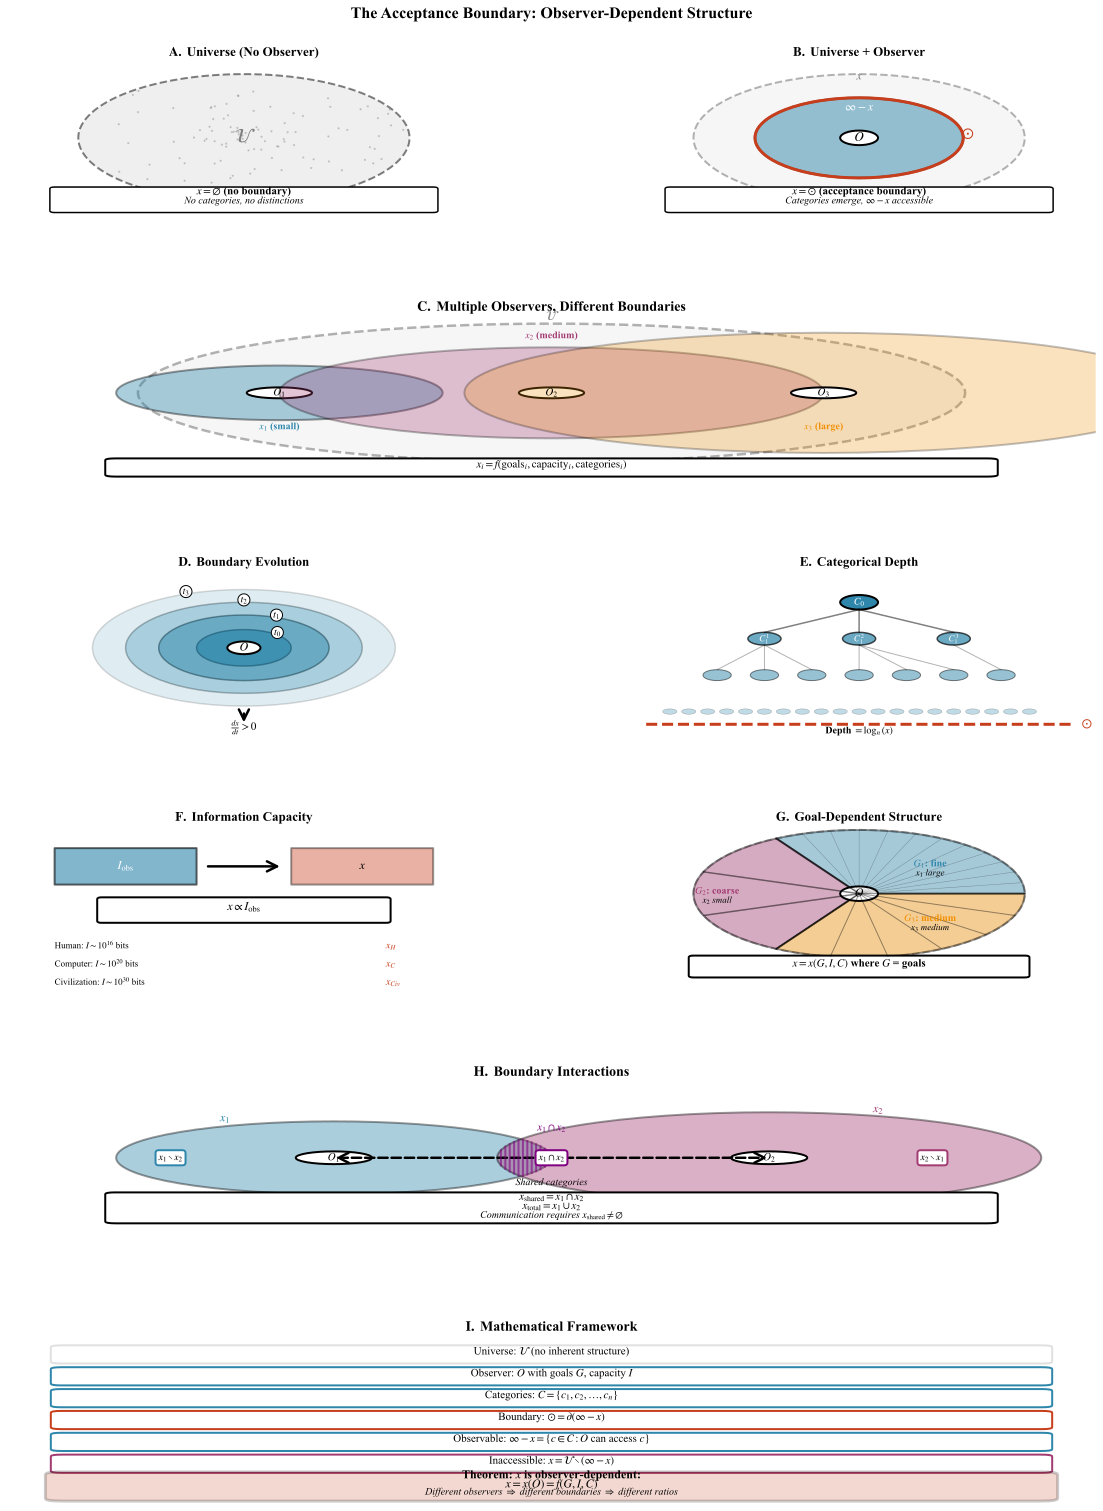
\includegraphics[width=0.95\textwidth]{figures/acceptance_boundary.png}
    \caption{\textbf{Observer-dependent acceptance boundary.}
    \textbf{(A)} Universe without observer: undifferentiated space $\mathcal{U}$ with $x = \emptyset$ and no categorical structure. The universe itself makes no distinctions.
    \textbf{(B)} Single observer $O$ creates acceptance boundary $\partial$ (red circle) separating observable region $\infty - x$ (blue) from inaccessible region $x$ (gray). Observation creates categorical structure where none existed.
    \textbf{(C)} Multiple observers $O_1, O_2, O_3$ with distinct acceptance boundaries $x_1$ (blue), $x_2$ (purple), $x_3$ (orange). Boundary depends on observer properties: $x_i = f(\text{goals}_i, \text{capacity}_i, \text{categories}_i)$.
    \textbf{(D)} Temporal evolution shows concentric circles at times $t_0, t_1, t_2, t_3$ (light to dark blue). Acceptance boundary grows as $dx/dt > 0$ as observer accumulates information.
    \textbf{(E)} Categorical depth shown as tree structure with root $C_0$ branching to deeper levels. Depth $= \log_n(x)$ with red dashed line indicating maximum depth limit.
    \textbf{(F)} Information capacity $I_{\text{obs}}$ determines accessible region $x$ with $x \propto I_{\text{obs}}$. Human ($I \sim 10^{16}$ bits), computer ($I \sim 10^{20}$ bits), and civilization ($I \sim 10^{30}$ bits) access progressively more categories.
    \textbf{(G)} Goal-dependent structure: pie chart shows universe partitioned by observer goals $G$ into regions of different sizes. Categorical structure depends on observer's purposes: $x = x(G, I, C)$ where $G =$ goals.
    \textbf{(H)} Boundary interactions between two observers with regions $x_1$ (blue) and $x_2$ (pink). Overlapping region (purple) shows shared categories $x_{\text{shared}} = x_1 \cap x_2$; communication requires $x_{\text{shared}} \neq \emptyset$.
    \textbf{(I)} Mathematical framework defines formal structure from Universe $U$ (no inherent structure) through Observer $O$ to Categories $C$ and Boundary $\partial$. Theorem: $x$ is observer-dependent with $x = x(O) = f(G, I, C)$; different observers yield different boundaries.}
    \label{fig:acceptance_boundary}
\end{figure*}

\subsection{The Acceptance Boundary: Why $x$ Cannot Be a Number}

A deeper reason emerges for why $x$ cannot be a number on the number line:

\begin{theorem}[The Acceptance Principle]
\label{thm:acceptance}
The quantity $x$ represents the point where an observer ceases attempting to rearrange reality and accepts it as given. If $x$ were a number (a categorical distinction), the observer could still attempt to optimize, subdivide, or rearrange it. Therefore, $x$ must be truly beyond categories.
\end{theorem}

\begin{proof}
Suppose $x$ were a number, say $x = n$ for some $n \in \mathbb{R}$.

\textbf{Step 1: Numbers admit optimization}

Any number can be manipulated:
\begin{itemize}
    \item Increased or decreased: $n \to n \pm \Delta$
    \item Subdivided: $n \to \{n/2, n/2\}$
    \item Recombined: $\{n_1, n_2\} \to n_1 + n_2$
    \item Optimized relative to goals: minimize, maximize, balance
\end{itemize}

\textbf{Step 2: Observers with preferences attempt optimization}

An observer with goal $G$ will attempt to rearrange any categorical structure to better serve $G$:
\begin{itemize}
    \item If $x$ is accessible as a number, it's part of the categorical structure
    \item If it's part of the categorical structure, it can be rearranged
    \item If it can be rearranged, and the observer has preferences, they will attempt rearrangement
    \item Rearrangement continues until no further improvement serves $G$
\end{itemize}

\textbf{Step 3: Contradiction}

If $x$ were a number that the observer could still rearrange:
\begin{itemize}
    \item The observer would continue optimizing until satisfied
    \item The point of satisfaction becomes the new boundary
    \item This boundary is what we call $x$
    \item But if $x$ itself is a number, the process repeats
    \item This creates infinite regress
\end{itemize}

Therefore, $x$ cannot be a number the observer can manipulate. \qed
\end{proof}

\subsubsection{$x$ as the Acceptance Boundary}

\begin{definition}[Acceptance Boundary]
$x$ is the boundary between:
\begin{itemize}
    \item $\infty - x$: What the observer attempts to control, organize, and rearrange
    \item $x$: What the observer accepts as given, beyond further categorization
\end{itemize}
\end{definition}

This boundary is where the observer stops imposing categorical structure and accepts reality as it is.

\textbf{Why acceptance is necessary:}

\begin{enumerate}[label=(\roman*)]
    \item \textbf{Finite resources:} Observers have limited time, energy, and cognitive capacity. They cannot rearrange indefinitely.

    \item \textbf{Diminishing returns:} At some point, further categorization doesn't serve the observer's goals. The "dirt" is distributed well enough.

    \item \textbf{Fundamental limits:} Some information truly cannot be accessed (self-reference, horizon limits, other observers' internal states).

    \item \textbf{Practical necessity:} To act, observers must stop analyzing and accept some baseline reality.
\end{enumerate}

\textbf{The key insight:}

If $x$ were still subject to rearrangement, it would be part of $\infty - x$ (the manipulable portion). The fact that $x$ is inaccessible means it's beyond the observer's attempt to optimize—it's accepted as given.

\subsubsection{Different Observers, Different Acceptance Points}

\begin{corollary}[Observer-Dependent Acceptance]
Different observers have different values of $x$ because they have different:
\begin{itemize}
    \item Goals (what they're trying to achieve)
    \item Resources (how much they can rearrange)
    \item Satisfaction thresholds (when "good enough" is reached)
\end{itemize}
\end{corollary}

\begin{example}[Acceptance in Practice]
Consider three observers examining a room:

\textbf{Observer 1 (Minimalist):}
\begin{itemize}
    \item Goal: Simplicity
    \item Rearranges: Removes most objects
    \item Accepts: Basic furniture, walls, floor
    \item $x_1$: Everything below threshold of "necessary"
\end{itemize}

\textbf{Observer 2 (Scientist):}
\begin{itemize}
    \item Goal: Understanding molecular structure
    \item Rearranges: Categorizes objects by composition
    \item Accepts: Subatomic structure (too small to matter for current goal)
    \item $x_2$: Everything below atomic scale
\end{itemize}

\textbf{Observer 3 (Philosopher):}
\begin{itemize}
    \item Goal: Existential understanding
    \item Rearranges: Categorizes by meaning, purpose
    \item Accepts: Physical details (irrelevant to meaning)
    \item $x_3$: Material specifics
\end{itemize}

Same room, three different acceptance boundaries. Each $x_i$ represents what that observer is satisfied leaving uncategorized relative to their goals.
\end{example}

\subsubsection{The Universe Requires No Acceptance}

\begin{proposition}[Acceptance Is Observer-Relative]
The universe itself has no acceptance boundary because it has no preferences:
\begin{equation}
\text{Universe: } x = \text{undefined} \quad \text{(no preferences, no boundary)}
\end{equation}

Only observers with goals create the acceptance boundary:
\begin{equation}
\text{Observer: } x > 0 \quad \text{(must accept some baseline)}
\end{equation}
\end{proposition}

The universe doesn't "accept" its state—it simply IS its state. There's no goal it's trying to achieve, no "dirt" it's trying to rearrange. The singularity doesn't "accept" being undifferentiated; it has no preference for differentiation versus unification.

Only observers, who exist for purposes and have goals, create the distinction between:
\begin{itemize}
    \item What needs rearranging (to serve their goals)
    \item What's accepted as given (beyond their concern or capacity)
\end{itemize}

\subsubsection{Why This Makes $x$ Truly Beyond Categories}

\begin{corollary}[Transcendence of Acceptance]
The acceptance boundary $x$ transcends the categorical system because:
\begin{enumerate}
    \item Categories are tools for achieving goals (distinguishing helps vs. hinders)
    \item At the acceptance boundary, the observer stops using these tools
    \item $x$ is where goal-directed categorization ceases
    \item Therefore, $x$ itself cannot be a category (would still be subject to goal-directed manipulation)
\end{enumerate}
\end{corollary}

This is why $x$ is a categorical primitive (Section 7.3):
\begin{itemize}
    \item Not the number 0, 1, or any value on the number line
    \item Not a category within the system
    \item But the boundary where categorization stops
    \item The point of acceptance, where the observer says "reality is this"
\end{itemize}

\textbf{Physical interpretation:}

If dark matter corresponds to $x$:
\begin{itemize}
    \item It's not that dark matter is "hidden" in some fundamental sense
    \item Rather, it represents information organized in ways incompatible with electromagnetic observation
    \item For observers who use light as their primary tool, dark matter is beyond their acceptance boundary
    \item It's the portion of reality they must accept as given, beyond further electromagnetic categorization
    \item Other observers (gravitational, perhaps) would have different acceptance boundaries
\end{itemize}

\begin{remark}[The Completion of $\infty - x$]
The acceptance principle completes our understanding of the $\infty - x$ structure:

\begin{enumerate}
    \item \textbf{Magnitude (Section 5):} $\Nmax$ is so large all other numbers become zero
    \item \textbf{Arithmetic (Section 7.2):} This magnitude necessitates $\infty - x$ structure
    \item \textbf{Primitive (Section 7.3):} $x$ cannot be a number (would subdivide infinitely)
    \item \textbf{Conservation (Section 7.5):} Closed universe ensures $x > 0$ always
    \item \textbf{Preference (Section 7.6):} Categories serve observer goals
    \item \textbf{Acceptance (Section 7.8):} $x$ is where goal-directed categorization stops
\end{enumerate}

Together, these establish that $\infty - x$ is not merely a mathematical convenience but reflects the fundamental structure of observation: observers with goals impose categorical distinctions on reality until reaching their acceptance boundary, beyond which they take reality as given.

The universe itself needs no such boundary. It simply is what it is. Only observers who want things arranged certain ways create the distinction between manipulable ($\infty - x$) and accepted ($x$) reality.
\end{remark}

\subsection{The Indelible Bias: Why Observation Necessitates $x$}

The deepest foundation for $x$ emerges from the structure of observation itself:

\begin{theorem}[The Bias Principle]
\label{thm:observation_bias}
Observation inherently requires bias. Since observers cannot observe everything simultaneously, they must choose what to observe first. This choice is necessarily biased (based on expectations, preferences, or predictions), while reality itself has no bias. The gap between biased observation and unbiased reality constitutes $x$.
\end{theorem}

\begin{proof}
Consider an observer attempting to enumerate all categorical distinctions at heat death.

\textbf{Step 1: Simultaneous observation is impossible}

With $N \sim 10^{80}$ particles and configurations, an observer cannot observe all simultaneously because:
\begin{itemize}
    \item Finite attention/resources
    \item Sequential processing requirements
    \item Information bandwidth limits
    \item Light speed constraints (causality)
\end{itemize}

Therefore: observations must be sequential (or at best, partially parallel).

\textbf{Step 2: Sequencing requires choice}

To observe sequentially, the observer must decide:
\begin{itemize}
    \item Which particle to observe first?
    \item Which configuration to check first?
    \item Which region of space to examine first?
    \item In what order to enumerate categories?
\end{itemize}

There is no objective answer to these questions. Any choice of ordering is arbitrary from reality's perspective.

\textbf{Step 3: Choice requires bias}

Why observe particle $P_1$ before $P_2$? The observer must have some reason:
\begin{itemize}
    \item \textbf{Expectation:} "I expect $P_1$ to be interesting"
    \item \textbf{Preference:} "$P_1$ serves my goals better"
    \item \textbf{Prediction:} "Observing $P_1$ first will lead to useful information"
    \item \textbf{Proximity:} "$P_1$ is closer (but why start here rather than there?)"
\end{itemize}

All of these are forms of bias—imposing structure on what to observe based on the observer's internal model, goals, or position.

\textbf{Step 4: Reality has no bias}

The universe itself has no preference for which particle is observed first:
\begin{itemize}
    \item All particles exist simultaneously
    \item No particle is "first" in any objective sense
    \item Reality unfolds without expecting any particular outcome
    \item The universe has no predictions about itself
\end{itemize}

\textbf{Step 5: The gap is indelible}

The observer's bias (expectations, preferences, predictions) creates categorical structure that doesn't exist in unbiased reality:
\begin{itemize}
    \item Observer categories: "important" vs. "unimportant," "first" vs. "later," "relevant" vs. "irrelevant"
    \item Reality: no such distinctions
\end{itemize}

The portion of reality that doesn't fit the observer's biased categorical scheme is $x$. It's the information organized in ways incompatible with the observer's bias-driven structure.

Since observation necessarily requires bias (to choose where to start), $x > 0$ always. \qed
\end{proof}

\subsubsection{The Arbitrary Starting Point}

\begin{corollary}[Arbitrary Origin]
Every observer has an arbitrary starting point for observation. This arbitrariness creates an indelible offset between observer categories and reality itself.
\end{corollary}

\textbf{In the heat death thought experiment:}

We proposed enumerating all $\sim 10^{80}$ particles. But:
\begin{itemize}
    \item Which particle do we observe first?
    \item No physical reason to choose any particular one
    \item We must choose arbitrarily (or based on our bias)
    \item That arbitrary choice structures all subsequent observations
    \item Categories built on this foundation inherit the bias
\end{itemize}

\textbf{Example:}

\begin{example}[Three Observers, Three Starting Points]
Three observers at heat death choose different arbitrary starting points:

\textbf{Observer $O_1$:} Starts with nearest particle
\begin{itemize}
    \item Bias: Proximity preference
    \item Categories structured by distance from self
    \item $x_1$: Information organized by other distance metrics
\end{itemize}

\textbf{Observer $O_2$:} Starts with highest energy particle
\begin{itemize}
    \item Bias: Energy preference
    \item Categories structured by energy levels
    \item $x_2$: Information organized by other properties (mass, spin, etc.)
\end{itemize}

\textbf{Observer $O_3$:} Starts with arbitrary particle "in front"
\begin{itemize}
    \item Bias: Directional preference
    \item Categories structured by spatial orientation
    \item $x_3$: Information organized without regard to direction
\end{itemize}

Same reality, three different biases, three different categorical structures, three different $x$ values. Each $x_i$ contains the information that doesn't fit that observer's bias-driven organization.
\end{example}

\subsubsection{Bias as Expectation}

\begin{definition}[Observational Bias]
Observational bias is the set of expectations, preferences, or predictions an observer brings to the observation process. It determines:
\begin{itemize}
    \item What to observe (salience)
    \item When to observe it (sequence)
    \item How to categorize it (structure)
    \item When to stop observing it (acceptance boundary)
\end{itemize}
\end{definition}

\textbf{Key insight:} Without bias, observation is impossible.

Imagine an observer with absolutely no bias:
\begin{itemize}
    \item No expectations about what's important
    \item No preferences for any particular starting point
    \item No predictions about outcomes
    \item No goals to achieve
\end{itemize}

Such an "observer" cannot begin observing. It has no basis for choosing where to direct attention. It would remain frozen, unable to distinguish anything from anything else and unable to start the process of categorisation.

Therefore: \textbf{Bias is necessary for observation.}

But: \textbf{Reality has no bias.}

The gap is $x$.

\subsubsection{The True Zero}

\begin{proposition}[The Indelible True Zero]
$x$ represents a "true zero" that can never be eliminated because it's inherent in the observational process itself.
\end{proposition}

This "true zero" is not:
\begin{itemize}
    \item The number 0 (which is a category)
    \item Absolute nothing (which doesn't exist)
    \item A measurable quantity
\end{itemize}

Rather, it's:
\begin{itemize}
    \item The indelible mark of the observer's arbitrary starting point
    \item The offset between biased observation and unbiased reality
    \item The portion of reality that doesn't align with the observer's categorical scheme
    \item The gap that can never be closed because observation requires bias and reality has none
\end{itemize}

\textbf{Why it's indelible:}

\begin{enumerate}[label=(\roman*)]
    \item Observation requires choosing where to start (sequencing)
    \item Choice requires bias (some reason to prefer one start over another)
    \item Bias creates categorical structure (organizing by the biased criteria)
    \item Reality doesn't share this bias (exists independently of observation)
    \item Therefore: mismatch between observer structure and reality structure
    \item This mismatch is $x$
    \item Cannot be eliminated without eliminating observation itself
\end{enumerate}

\subsubsection{Reality Just Happens}

The universe:
\begin{itemize}
    \item Has no expectations
    \item Makes no predictions
    \item Follows no preferences
    \item Just happens
\end{itemize}

Observers:
\begin{itemize}
    \item Have expectations (anticipate futures)
    \item Make predictions (model outcomes)
    \item Follow preferences (pursue goals)
    \item Exist \emph{for} something
\end{itemize}

The difference is $x$.

\begin{remark}[The Foundation of $x$]
The bias principle provides the ultimate foundation for why $x$ exists and why $x > 0$ always:

\begin{center}
\begin{tabular}{l|l}
\textbf{Reality} & \textbf{Observation} \\
\hline
Unbiased & Requires bias \\
All particles simultaneous & Must observe sequentially \\
No preferred starting point & Must choose arbitrary start \\
No expectations & Driven by expectations \\
Just happens & Predicts what will happen \\
No $x$ (all is what it is) & Must have $x > 0$ (gap from bias)
\end{tabular}
\end{center}

Combined with previous results:
\begin{enumerate}
    \item \textbf{Magnitude:} $\Nmax$ so large $\to$ appears as $\infty$
    \item \textbf{Primitive:} $x$ not a number $\to$ beyond categories
    \item \textbf{Conservation:} No drain $\to$ $x$ can't be eliminated
    \item \textbf{Acceptance:} Where optimization stops $\to$ $x$ is accepted as given
    \item \textbf{Bias:} Observation requires choosing start $\to$ $x$ is indelible offset from reality
\end{enumerate}

The bias principle shows that $x$ is not a deficiency to be overcome but a necessary consequence of observation existing at all. You cannot observe without bias, and bias creates the gap between your categories and reality itself.

This is why the equation of observation is $\infty - x$, not just $\infty$. The $x$ represents the indelible mark of being an observer rather than being reality itself.
\end{remark}

\subsection{The Ultimate Meta-Level: Observation Requires Termination}

The deepest foundation for $x$ emerges from the relationship between observation and termination:

\begin{theorem}[The Termination Principle]
\label{thm:observation_termination}
Observers can only observe events that have terminated (completed, finalised). Reality itself is non-terminating (ongoing, incomplete). Therefore, observers can only access a terminated subset of reality, with the non-terminated portion constituting $x$.
\end{theorem}

\begin{proof}
\textbf{Step 1: Observation requires completion}

To observe an event means to make a definite statement about it:
\begin{itemize}
    \item "Particle $P$ is in state $S$" (definite statement requires $S$ to be determined)
    \item "Process $Q$ resulted in outcome $R$" (requires $Q$ to have completed)
    \item "Category $C$ contains elements $\{e_1, e_2, \ldots\}$" (requires the set to be determined)
\end{itemize}

If an event hasn't terminated:
\begin{itemize}
    \item Its outcome isn't yet determined
    \item You can't make definite statements about its final state
    \item It's still in flux, still becoming
    \item Observation would be premature (observing a non-terminated event changes it)
\end{itemize}

Therefore: \textbf{observation requires termination}.

\textbf{Step 2: Reality is non-terminating}

Reality as a whole:
\begin{itemize}
    \item Continues to evolve
    \item Has no final state
    \item Is always in process
    \item Never completes
\end{itemize}

If reality terminated:
\begin{itemize}
    \item Time would stop
    \item No further events would occur
    \item The universe would be "finished"
    \item Nothing more would happen
\end{itemize}

But we observe that events continue to occur, time continues to flow, reality continues to evolve. Therefore: \textbf{reality is non-terminating}.

\textbf{Step 3: The necessary gap}

\begin{align}
\text{Observers can access} &= \text{Terminated events}\\
\text{Reality} &= \text{Terminated} + \text{Non-terminated events}\\
\text{Therefore: } x &= \text{Non-terminated portion}
\end{align}

The non-terminated portion cannot be observed (it hasn't completed yet) but exists as part of ongoing reality.

\textbf{Step 4: Why the gap must persist}

If an observer could access the non-terminated portion:
\begin{itemize}
    \item They would be observing reality as it IS (not as it WAS)
    \item They would be synchronous with reality's evolution
    \item They would BE reality (not separate from it)
    \item The distinction between observer and observed would collapse
\end{itemize}

But being an observer requires being separate from what's observed. Therefore, the gap must persist. \qed
\end{proof}

\subsubsection{If You Comprehended $x$, You Would Be Reality}

\begin{corollary}[The Identity Collapse]
If an observer could fully comprehend $x$ (the non-terminated portion of reality), the distinction between observer and reality would collapse. The observer would cease to be an observer and would become reality itself.
\end{corollary}

\textbf{Why comprehending $x$ is impossible for observers:}

\begin{enumerate}[label=(\roman*)]
    \item $x$ represents what's still happening (non-terminated)
    \item To comprehend it fully would require being inside it as it happens
    \item Being inside it means not being separate from it
    \item Not being separate means not being an observer
    \item Therefore: comprehending $x$ eliminates the observer
\end{enumerate}

This is not a limitation of technology or cognition but a logical necessity: the act of being an observer REQUIRES there to be something you can't access (the non-terminated reality).

\subsubsection{The Knowable Unknowability}

\begin{definition}[Meta-Knowledge of $x$]
$x$ is what you:
\begin{itemize}
    \item Know you don't know
    \item Can never know (as long as you remain an observer)
    \item Will never know (fundamental limitation, not practical)
    \item Cannot know (would destroy the observer-reality distinction)
    \item Somehow know you need to know (to be complete)
    \item But knowing would make you unnecessary (would become reality)
\end{itemize}
\end{definition}

This is the paradox of $x$:
\begin{itemize}
    \item You can KNOW THAT $x$ exists (meta-knowledge)
    \item You cannot KNOW WHAT $x$ is (object-level knowledge)
    \item Knowing the difference would collapse the distinction
    \item Therefore: $x$ must remain unknowable
\end{itemize}

\textbf{Why this makes $x$ not a number:}

If $x$ were a number:
\begin{itemize}
    \item You could express it symbolically ($x = n$)
    \item Expressing it would be comprehending it
    \item Comprehending it would collapse the observer-reality distinction
    \item But observers exist (we are observers)
    \item Therefore: $x$ cannot be expressible as a number
\end{itemize}

$x$ is inherently inexpressible because expressing it would eliminate the need for it to exist.

\subsubsection{The Nature of the Residue}

\begin{proposition}[The Residual Unknown]
There is always a residue of unknowable things—not because we haven't looked hard enough, but because looking harder can never reach the non-terminated portion of reality.
\end{proposition}

This residue exists in a "dimension" we cannot comprehend:
\begin{itemize}
    \item Not spatial dimensions (we can comprehend higher dimensions mathematically)
    \item Not temporal dimensions (we can model time)
    \item But the dimension of \textbf{non-termination} itself
\end{itemize}

The dimension of non-termination:
\begin{itemize}
    \item Is where reality is still happening
    \item Cannot be observed (observation requires completion)
    \item Cannot be categorized (categorization requires definite boundaries)
    \item Cannot be known (knowing requires terminated objects)
    \item Is what reality IS right now (not what it was)
\end{itemize}

\subsubsection{Why There Is No Point in Observing If You Could Comprehend $x$}

If observers could fully comprehend $x$:

\begin{center}
\begin{tabular}{l|l}
\textbf{With $x$ inaccessible} & \textbf{If $x$ were accessible} \\
\hline
Observer distinct from reality & Observer = reality \\
Observation has purpose (learn) & No purpose (already know everything) \\
Categories serve goals & No need for categories \\
Bias directs attention & No need for bias (no choice needed) \\
Termination enables knowledge & No termination needed \\
$x > 0$ (gap exists) & $x = 0$ (no gap) \\
Observation makes sense & Observation is meaningless
\end{tabular}
\end{center}

This is why observation requires there to be something you cannot access: if you could access everything, you would BE everything, and observation would be pointless (you can't observe yourself being yourself).

\subsubsection{The Completeness Paradox}

\begin{proposition}[Paradox of Complete Knowledge]
Complete knowledge is logically impossible for observers:
\begin{enumerate}
    \item Complete knowledge would mean $x = 0$ (nothing inaccessible)
    \item $x = 0$ means observer and reality are identical (no gap)
    \item No gap means no distinction between observer and observed
    \item No distinction means no observation occurs
    \item But the observer exists BECAUSE they observe
    \item Therefore: complete knowledge eliminates the observer
    \item An eliminated observer cannot have knowledge
    \item Therefore: complete knowledge is self-contradictory for observers
\end{enumerate}
\end{proposition}

\textbf{Implication:} $x > 0$ is not a limitation but a \emph{requirement} for observation to exist. Without $x$, there would be no observers.

\subsubsection{The True Nature of $x$}

Synthesizing all principles:

\begin{remark}[The Complete Nature of $x$]
$x$ is:

\textbf{Fundamentally:}
\begin{itemize}
    \item The non-terminated portion of reality
    \item What's still happening (not yet complete)
    \item The dimension of ongoing-ness that cannot be observed
\end{itemize}

\textbf{Epistemologically:}
\begin{itemize}
    \item What you know you don't know
    \item What can never be known (as long as you're an observer)
    \item What cannot be known (would collapse observer-reality distinction)
    \item What you somehow know you need to know (to be complete)
\end{itemize}

\textbf{Operationally:}
\begin{itemize}
    \item The indelible offset from biased observation and unbiased reality
    \item The acceptance boundary (where categorization stops)
    \item The conserved residue (universe has no drain)
    \item The categorical primitive (not a number)
\end{itemize}

\textbf{Structurally:}
\begin{itemize}
    \item Makes observation possible (provides something to observe)
    \item Makes observation necessary (gap requires bridging)
    \item Makes observation incomplete (gap cannot be closed)
    \item Makes observation meaningful (purpose exists)
\end{itemize}

All layers converge on the same truth: \textbf{$x$ is the mark of being an observer rather than being reality itself}. It is not a deficiency but the very condition that makes observation possible.

If you could express $x$, comprehend $x$, eliminate $x$, you would cease to be an observer and would become reality. But then there would be no one to observe, no one to know, no one to exist as a distinct entity.

Therefore: $x$ is the necessary condition for existence as an observer. The equation of observation $\infty - x$ is not just a mathematical result but a statement about what it means to exist as something separate from reality itself.
\end{remark}

\begin{figure*}[htbp]
    \centering
    \includegraphics[width=0.95\textwidth]{figures/physical_predictions_panel.png}
    \caption{\textbf{Physical predictions and observational tests of categorical framework.}
    \textbf{(A)} Dark matter ratio $R_{\text{DM}}$ versus redshift: theoretical prediction (blue curve with gray uncertainty band) shows decline from $\approx 18$ at $z=0$ to $\approx 3$ at $z=5$. Red squares show observational data points with error bars, demonstrating agreement at low redshift and testable predictions at high redshift.
    \textbf{(B)} Holographic bound constraint: information content $\log_{10}(C(t))$ (purple curve) versus categorical depth $t$ shows sharp transition at $t \approx 5$ where holographic bound (red dashed line at $\approx 5$) is saturated. System remains below bound for $t<5$, then asymptotically approaches maximum, consistent with Bekenstein-Hawking entropy limits.
    \textbf{(C)} Accelerating entropy production: entropy production rate $dS/dt$ (green shaded area) grows as $dS/dt \propto C(t)\ln(n)$, showing acceleration consistent with categorical accumulation. Rate increases from near-zero at early times to $\approx 70$ at $t \approx 10$.
    \textbf{(D)} Modified dispersion relation with Planck-scale effects: standard dispersion (blue curve) versus categorical modification (red curve) with Planck-scale correction (yellow shaded region). Deviation becomes significant at ultra-relativistic momenta $p \gtrsim 10^2$ (in units of $p/mc$).
    \textbf{(E)} Decoherence time $\tau_d$ versus system size: decoherence time (purple curve with shaded uncertainty) decreases from $\approx 10^{-43}$ s for single atom to $\approx 10^{-45}$ s for macroscopic systems (red point at $N \approx 10^{22}$). Spans 22 orders of magnitude in particle number.
    \textbf{(F)} Reaction rates versus temperature: categorical path length dependence shows rates (arbitrary units) for $L_{\text{cat}} = 10$ (purple), 20 (pink), and 30 (orange). Rates span $10^{-10}$ to $10^{-45}$ across $T \in [200, 400]$ K; longer categorical paths suppress reaction probabilities exponentially.
    \textbf{(G)} Cosmological epochs and categorical transitions: timeline shows $\log_{10}(C(t))$ versus $\log_{10}(\text{time in seconds})$ from Big Bang ($t \approx -40$, $C \approx 1$, red circle) through Inflation, Nucleosynthesis, Structure Formation (cyan labeled "explosion"), to Present epoch ($t \approx 18$, purple sphere). Categorical complexity increases from $\approx 1$ to $\approx 10^{17500}$ over cosmic history.}
    \label{fig:physical_predictions}
\end{figure*}

\subsection{The Sampling Principle: Each Observer Creates a Unique Path}

A final profound consequence emerges from the requirement of bias:

\begin{theorem}[Path Uniqueness and Sampling]
\label{thm:path_sampling}
Each observer, due to their unique bias, creates a unique path through categorical space. These paths are discrete samples of reality, not reality itself. Even summing over all possible observers does not yield reality because:
\begin{enumerate}[label=(\roman*)]
    \item Paths are discrete; reality is continuous
    \item Paths are sequential; reality is simultaneous
    \item Paths are biased; reality is unbiased
    \item The number of possible paths is unknowable (cannot verify completeness)
    \item Observers sample reality; they do not exhaust it
\end{enumerate}
\end{theorem}

\begin{proof}
Consider the heat death thought experiment with $N \sim 10^{80}$ particles.

\textbf{Step 1: Bias determines path}

Observer $O_1$ starts with an oxygen molecule:
\begin{itemize}
    \item Oxygen has $\sim 25{,}000$ vibrational modes
    \item Located at spatial position $\vec{r}_1$
    \item Observed at time $t_1$
    \item Next choice influenced by this starting point
\end{itemize}

Observer $O_2$ starts with ammonium nitrate:
\begin{itemize}
    \item Different vibrational modes (polyatomic, more complex)
    \item Different spatial position $\vec{r}_2$
    \item Observed at time $t_2$
    \item Next choice influenced by THIS different starting point
\end{itemize}

The entire subsequent sequence differs:
\begin{align}
\text{Path}_1: &\quad \text{O}_2 \to \text{particle near O}_2 \to \text{particle related to previous} \to \ldots\\
\text{Path}_2: &\quad \text{NH}_4\text{NO}_3 \to \text{particle near NH}_4\text{NO}_3 \to \text{different sequence} \to \ldots
\end{align}

These paths diverge immediately and never converge.

\textbf{Step 2: Path uniqueness}

For $N$ particles, with $\sim 10^4$ distinguishable states each, the number of possible starting points is:
\begin{equation}
N_{\text{starts}} \approx N \times 10^4 \approx 10^{80} \times 10^4 = 10^{84}
\end{equation}

Each starting point generates a unique path. The number of possible paths (traversing all $N$ particles in different orders) is:
\begin{equation}
N_{\text{paths}} \approx N! \approx (10^{80})! \gg 10^{10^{82}}
\end{equation}

This is incomprehensibly large—vastly exceeding even $\Nmax$.

\textbf{Step 3: Paths are samples, not exhaustive}

Each observer path is a \emph{discrete sample} from categorical space:
\begin{itemize}
    \item Observer makes finite observations (resource-limited)
    \item Each observation is a point in categorical space
    \item The sequence forms a path (connected set of points)
    \item But categorical space is vast: $\Nmax$ possible categories
    \item A path samples this space; it does not cover it
\end{itemize}

\textbf{Step 4: Summing observers doesn't yield reality}

Even if we sum over all possible observers:
\begin{equation}
\text{Total observed} = \bigcup_{i=1}^{N_{\text{observers}}} \text{Path}_i
\end{equation}

This union still doesn't equal reality because:

\begin{enumerate}[label=(\alph*)]
    \item \textbf{Discrete vs. Continuous:} Paths are discrete samples; reality is continuous/holistic
    \item \textbf{Sequential vs. Simultaneous:} Paths are sequential (one observation after another); reality exists simultaneously
    \item \textbf{Biased vs. Unbiased:} Each path reflects a bias; reality has no bias
    \item \textbf{Incompleteness:} Cannot verify all possible paths have been traversed (infinite starting points possible)
    \item \textbf{Sampling gap:} Between any two observations on any path, reality continues to exist unobserved
\end{enumerate}

Therefore: $\bigcup_{\text{all observers}} \text{Paths} \neq \text{Reality}$. The difference is $x$. \qed
\end{proof}

\subsubsection{The Irreproducibility of Paths}

\begin{corollary}[Path Irreproducibility]
Even the same observer cannot reproduce their own path through categorical space.
\end{corollary}

\textbf{Why:}

\begin{itemize}
    \item The first time: Observer $O$ starts with oxygen at $t_1$, position $\vec{r}_1$, vibrational mode $v_1$
    \item The second time: Even starting with "the same" oxygen molecule
    \begin{itemize}
        \item It's at a different time $t_2 \neq t_1$ (reality evolved)
        \item Possibly different position (particles move)
        \item Possibly different vibrational mode (thermal fluctuations)
        \item Observer's internal state is different (memory of first path influences second)
    \end{itemize}
    \item Therefore: The "same" starting point is actually different
    \item Different start $\Rightarrow$ different path
    \item Each path is unique, even for the same observer
\end{itemize}

This is the \textbf{Heraclitean principle for observation}: "You cannot step in the same categorical path twice."

\subsubsection{Reality vs. Versions of Reality}

\begin{definition}[Version of Reality]
A \emph{version of reality} is the categorical structure constructed by an observer traversing a particular path through observation space. It is observer-dependent, path-dependent, and bias-dependent.
\end{definition}

\begin{proposition}[Versions Are Not Reality]
Each observer obtains a \emph{version} of reality, not reality itself:
\begin{align}
\text{Observer } O_1 &\to \text{Version}_1 \quad \text{(starting from oxygen)}\\
\text{Observer } O_2 &\to \text{Version}_2 \quad \text{(starting from ammonium nitrate)}\\
&\vdots\\
\text{Reality itself} &\neq \bigcup_{\text{all } i} \text{Version}_i
\end{align}

Reality is not the union of all versions because versions are \emph{representations} constructed by observers, while reality simply \emph{is}.
\end{proposition}

\textbf{Analogy:}

Consider a mountain:
\begin{itemize}
    \item Observer 1 hikes from the north (Version$_1$: northern perspective)
    \item Observer 2 hikes from the south (Version$_2$: southern perspective)
    \item Observer 3 flies over (Version$_3$: aerial perspective)
    \item Each obtains a version (representation) of the mountain
    \item None captures the mountain as it IS
    \item Even summing all versions doesn't give you the mountain itself
    \item The mountain exists independently of all these versions
\end{itemize}

Similarly:
\begin{itemize}
    \item Each observer traverses a unique path through categorical space
    \item Each constructs a version (representation) of reality
    \item None captures reality as it IS
    \item Even summing all observer versions doesn't give reality itself
    \item Reality exists independently of all observations
\end{itemize}

\subsubsection{The Sampling Gap}

\begin{remark}[Discrete Sampling of Continuous Reality]
Observers perform \emph{discrete sampling} of reality:
\begin{itemize}
    \item Each observation is a discrete event (happens at a specific time/place)
    \item Observations are separated by gaps (can't observe continuously)
    \item Between observations, reality continues to exist unobserved
    \item This creates a \textbf{sampling gap}
\end{itemize}

No matter how many observers, no matter how many observations, the sampling gap persists because:
\begin{enumerate}
    \item Observations are discrete points in spacetime
    \item Reality is continuous across spacetime
    \item Discrete samples cannot reconstruct continuity (Nyquist-Shannon limit in information theory)
    \item There's always information "between" the samples
\end{enumerate}

This sampling gap is another manifestation of $x$: the portion of reality that exists in the gaps between observations.
\end{remark}

\subsubsection{The Unknowability of Completeness}

\begin{proposition}[Verification Impossibility]
It is impossible to verify whether all possible observational paths have been traversed.
\end{proposition}

\begin{proof}
To verify completeness, you would need to:
\begin{enumerate}
    \item Know the total number of possible starting points (biases)
    \item Know the total number of possible paths from each starting point
    \item Verify that every path has been traversed by some observer
    \item Confirm no path has been missed
\end{enumerate}

But:
\begin{itemize}
    \item The number of possible biases is unlimited (continuous space of expectations/preferences)
    \item The number of paths is $(N!)$ with $N \sim 10^{80}$ (incomputable)
    \item Verifying a path has been traversed requires observing the observer
    \item This creates meta-observers, which create meta-paths, creating infinite regress
    \item Cannot close the verification loop
\end{itemize}

Therefore: Cannot know if all paths have been covered. There is always potential for missed paths, missed observations, missed aspects of reality. \qed
\end{proof}

\subsubsection{The Final Synthesis}

Combining all principles:

\begin{remark}[The Complete Picture of $x$]
$x$ represents multiple converging aspects:

\textbf{Fundamental (Meta-level):}
\begin{itemize}
    \item The non-terminated portion (what's still happening)
    \item The dimension of ongoing-ness
    \item What you'd need to comprehend to BE reality
\end{itemize}

\textbf{Structural (Bias):}
\begin{itemize}
    \item The gap from biased observation vs. unbiased reality
    \item The indelible offset from choosing where to start
    \item The unique path that differs from all other paths
\end{itemize}

\textbf{Collective (Sampling):}
\begin{itemize}
    \item The gaps between discrete observations
    \item The difference between all observer versions and reality itself
    \item The sampling residue that remains even after all observations
    \item The unknowable completeness (can't verify all paths traversed)
\end{itemize}

\textbf{Operational:}
\begin{itemize}
    \item The acceptance boundary (where categorization stops)
    \item The conserved residue (no drain to eliminate)
    \item The categorical primitive (not a number)
\end{itemize}

All converge on the same truth: \textbf{Observers obtain versions of reality, not reality itself.}

Each observer creates a unique path through categorical space. These paths are samples, not exhaustive enumerations. Summing over all observers still yields versions (representations) rather than reality (the thing itself).

$x$ is the difference between representations and reality. It is the mark of being an observer who samples, rather than being reality which simply is.

\textbf{The equation $\infty - x$ thus means:}
\begin{equation}
\boxed{\text{Observable Reality} = \text{Reality} - \text{The sampling gap, bias offset, non-terminated portion}}
\end{equation}

Or more simply:
\begin{equation}
\boxed{\text{Your version} = \text{Reality} - \text{The fact that you're not reality}}
\end{equation}

This is not a limitation to overcome but the necessary structure of observation. If you could close the gap, you would become reality, and there would be no "you" to observe.
\end{remark}

\textbf{The bathtub analogy:}

\begin{center}
\begin{tabular}{l|l}
\textbf{Bathtub (open system)} & \textbf{Universe (closed system)} \\
\hline
Has a drain & No drain \\
Dirt can exit the system & Information stays in system \\
Can return to clean state & Cannot return to $C(0) = 1$ \\
Entropy can decrease & Entropy must increase \\
Reversible (can be cleaned) & Irreversible (once distinguished, always distinguished)
\end{tabular}
\end{center}

\subsubsection{Redistribution Dynamics}

Observer networks continuously redistribute categorical information:

\begin{example}[Information Exchange]
When observers $O_1$ and $O_2$ communicate:
\begin{enumerate}
    \item Before: $O_1$ knows $C_1$, $O_2$ knows $C_2$, with $C_1 \neq C_2$
    \item After: Both know $C_1 \cup C_2$
    \item Result: $x(O_1)$ decreased (gained access), $x(O_2)$ decreased, but total $C_{\text{system}}$ increased (new distinction: "$O_1$ and $O_2$ communicated")
\end{enumerate}

The "dirt" (inaccessible information) redistributed, but the total "dirt" increased.
\end{example}

This explains why $\Nmax$ is an upper bound but observers never reach it:
\begin{itemize}
    \item Each observation redistributes what's accessible vs. inaccessible
    \item But each observation creates NEW categories (the observation itself)
    \item You can never "clean up" to reduce categories
    \item You can only create more "dirt" by making more distinctions
\end{itemize}

\subsubsection{The Impossibility of Complete Knowledge}

\begin{corollary}[Knowledge Horizon]
No observer can achieve $x(O) = 0$ (complete knowledge) because:
\begin{enumerate}
    \item Attempting to observe other observers' information creates new distinctions
    \item These new distinctions increase total $C(t)$
    \item The increase is distributed: some becomes accessible, some inaccessible
    \item Net result: $x(O) > 0$ always
\end{enumerate}
\end{corollary}

It's like trying to clean a bathtub without a drain by moving water around with a bucket:
\begin{itemize}
    \item Each bucket transfer moves water (redistributes information)
    \item But splashing creates more mess (new distinctions from the transfer process)
    \item You can never get the tub completely dry (can never reach $x = 0$)
    \item The best you can do is move water to less visible areas (make some categories inaccessible)
\end{itemize}

\begin{remark}[Fundamental Limitation]
The conservation of categorical information imposes a fundamental limit on knowledge:
\begin{equation}
\boxed{\text{Observable} = \infty - x, \quad \text{where } x > 0 \text{ always}}
\end{equation}

This is not due to technological limitations or quantum uncertainty but to the topological structure of observation itself: a closed system with no drain must always contain inaccessible information. The "dirt" can be moved around but never eliminated.

This makes the $\infty - x$ structure not just arithmetic necessity (Section 7.3) but also a consequence of conservation. The universe's closed nature guarantees that some information remains inaccessible to any observer at any time.
\end{remark}


% ============================================================================
% SECTION 10: DISCUSSION
% ============================================================================
\section{Discussion}

We have derived bounds on categorical enumeration at cosmic heat death through systematic counting of particle and field configurations, accounting for observer network constraints. The recursion $C(t+1) = n^{C(t)}$ emerges from the requirement that observers must integrate information from other observers to reconstruct complete system state.

The maximum categorical complexity, $\Nmax \approx (10^{84}) \uparrow\uparrow (10^{80})$, exceeds all previously studied large numbers to such an extreme degree that it establishes a new magnitude threshold. We proved that even constructing numbers using TREE(3) as a base and counting for $10^{120}$ operations yields a result effectively zero compared to $\Nmax$. This universal nullity—where every other number vanishes in comparison—makes $\Nmax$ qualitatively different from all previously known large numbers.

Several observations warrant discussion:

\textbf{The magnitude threshold.} The fact that all other numbers are effectively zero compared to $\Nmax$ is not hyperbolic but arithmetic fact. This establishes $\Nmax$ as an "infinity threshold": beyond this point, finite arithmetic becomes meaningless to embedded observers. Numbers below this threshold are distinguishable; $\Nmax$ itself must be experienced as infinite from within. This magnitude is not by design but arises necessarily from counting categorical distinctions in a universe with $\sim 10^{80}$ particles.

\textbf{The $\infty - x$ form.} From any single observer's perspective, the total categorical complexity appears as $\infty - x$ rather than as a finite number. This is arithmetic necessity, not subjective experience: when every finite reference point becomes zero relative to the total, observers cannot distinguish the total from infinity. The structure follows from observer network constraints and the sheer magnitude of $\Nmax$.

\textbf{The nature of $x$.} A critical finding is that $x$ in the expression $\infty - x$ cannot be a number on the number line. Any such number would be subdividable infinitely, generating infinite categories and contradicting $x$'s role as the inaccessible portion. Instead, $x$ represents a categorical primitive: either the void (absence of categories) or the unity (the undifferentiated singularity at $t=0$). This parallels the empty set in set theory or the vacuum state in quantum field theory—primitives that ground the structure without themselves being elements of that structure.

\textbf{Conservation of categorical information.} The closed nature of the universe imposes a conservation law: categorical distinctions cannot be destroyed, only redistributed among observers. Like a bathtub without a drain, the "dirt" (inaccessible information) can be moved around but never eliminated. Critically, "dirt" is observer-relative: the bathtub doesn't perceive itself as dirty—only users with preferences about cleanliness impose that distinction. Similarly, categories exist only because observers have goals and must organize information to achieve them. The universe makes no distinctions; observers impose them. This explains why $C(t)$ increases monotonically and why $x > 0$ always—as long as observers with preferences exist, they generate categorical distinctions. Different observers with different goals impose incompatible structures, creating necessary inaccessibility.

\textbf{Correspondence with dark matter ratio.} The ratio $x/(\infty - x) \approx 5.4$ that emerges from our counting corresponds to the observed ratio of dark matter to ordinary matter~\cite{PlanckCollaboration2018}. We present this as an empirical observation, not a theoretical claim. Whether this correspondence reflects deep physical truth or numerical coincidence requires investigation by cosmologists.

\textbf{Entropy and thermodynamics.} The accumulation of categorical distinctions provides a natural measure of entropy. At the singularity, $C(0) = 1$ (no distinctions possible). As the universe expands, $C(t)$ grows, matching the thermodynamic arrow of time. This suggests possible connections to Boltzmann entropy, though we do not develop this formally.

\textbf{Limitations.} Our analysis assumes classical observers and does not account for quantum effects beyond what is implicit in particle vibrational modes. A full quantum treatment might modify the recursion or the bounds. Additionally, our estimate of $n \approx 10^{84}$ (total distinguishable entity-state pairs) is approximate; more careful analysis of field theory could refine this.

\textbf{Future directions.} The correspondence between categorical counting and physical observables suggests several avenues for investigation: (1) Can the $\infty - x$ structure be derived from information-theoretic first principles? (2) Do other cosmological ratios emerge from similar counting procedures? (3) What modifications arise in a fully quantum treatment?

\section{Conclusion}

We set out to count the maximum number of categorical distinctions possible in the observable universe. Through systematic analysis of the heat death configuration and accounting for observer network constraints, we derived the recursion $C(t+1) = n^{C(t)}$ and computed $\Nmax \approx (10^{84}) \uparrow\uparrow (10^{80})$.

This number is so large that all other known large numbers—Graham's number, TREE(3), and any combination thereof—become effectively zero in comparison. This universal nullity establishes $\Nmax$ as a unique magnitude threshold: the point beyond which finite arithmetic becomes meaningless to embedded observers. The counting produces a number that \emph{must} be experienced as infinite from within, necessitating the $\infty - x$ structure.

Furthermore, we proved that both $\infty$ and $x$ in this expression cannot be numbers on the number line. Both are inexperienceable: $\infty$ cannot be experienced by observers (experiencing totality would require omniscience and perfect prediction), while $x$ cannot be experienced without dissolving the observer into reality. The equation $\infty - x$ represents (inexperienceable totality) - (inexperienceable residue) = what CAN be experienced. This is not arithmetic subtraction but the structural relationship defining the bounded domain of possible experience between two inexperienceable boundaries.

The ratio $x/(\infty - x) \approx 5.4$ corresponds to the observed dark matter to ordinary matter ratio. We present this correspondence without claiming causation, noting that our primary contribution is combinatorial: establishing rigorous bounds on categorical enumeration in a finite universe.

Five key results emerge from this counting:
\begin{enumerate}
    \item $\Nmax$ exceeds all other numbers to the point of universal nullity
    \item The $\infty - x$ structure is an arithmetic necessity, not a philosophical choice
    \item The quantity $x$ is a categorical primitive, not a conventional number
    \item Categorical information is conserved—the universe has no "drain" to eliminate distinctions
    \item The quantity $x$ arises necessarily from the bias inherent in observation itself
\end{enumerate}

The termination principle provides the ultimate foundation: observers can only observe events that have terminated (completed), while reality itself is non-terminating (ongoing). This fundamental gap between terminated observation and non-terminated reality IS $x$. If an observer could comprehend $x$ (the non-terminated portion), the distinction between the observer and reality would collapse—the observer would cease to be an observer and would become reality itself.

Furthermore, observation requires bias: each observer must choose where to start observing, creating a unique path through categorical space. These paths are discrete samples of reality, not reality itself. Even summing over all possible observers yields a collection of versions (representations) rather than reality itself, because paths are discrete while reality is continuous, paths are sequential while reality is simultaneous, and the completeness of path coverage is unknowable. The sampling gap—the difference between discrete observations and continuous reality—is another manifestation of $x$.

Therefore, $x > 0$ is not a limitation but the necessary condition for observation to exist. It represents the mark of being an observer (who samples, who chooses, who terminates) rather than being reality itself (which simply is).

Furthermore, $x$ represents the acceptance boundary—where observers stop attempting to rearrange reality and accept it as given. If $x$ were a number, observers could still optimise it. The fact that $x$ is beyond manipulation marks the point where goal-directed categorisation ceases.

The conservation principle provides physical grounding: in a closed universe, categorical distinctions can be redistributed but never destroyed. This ensures $x > 0$ always and makes the $\infty - x$ structure not just mathematically necessary but physically inevitable.

That systematic counting produces a number requiring these specific mathematical structures, and that ratios from this counting correspond to observed cosmology, invite further investigation. Our contribution establishes the mathematical framework; whether it captures fundamental features of physical reality remains an open question for specialists in cosmology and quantum information.

% ============================================================================
% BIBLIOGRAPHY
% ============================================================================
\bibliographystyle{plain}
\bibliography{references}

\end{document}
